% IRAI 2027 regular paper (<= 6 pages incl. references, IEEE two-column, single-blind).
% Build: tectonic -X compile main.tex --outdir build (or latexmk -pdf). Result numbers are macros in generated/:
%   results_macros.tex (Qwen3, notebook 08), results_macros_llama.tex (prefix Llama), results_macros_block1.tex (prefix BlockOne),
%   all written by harness/analyze.py; posthoc_macros.tex (prefix Ph, post hoc and exploratory) written by harness/posthoc.py
%   (notebook 09). Never type a result number by hand; notebook 07 checks that generated/ matches the analysis outputs.
\documentclass[conference]{IEEEtran}
\IEEEoverridecommandlockouts
\usepackage[T1]{fontenc} % Times via Type 1 fonts under both pdfLaTeX and XeTeX (Tectonic)
\usepackage{cite}
\usepackage{amsmath,amssymb}
\usepackage{booktabs,tabularx}
\usepackage{graphicx}
\usepackage{url}
\usepackage{xstring}
% generated by harness/analyze.py from runs_dev_qwen3-8b.jsonl (sha256 5e8844bb83d32cfcbad9d0945ca50c827c06467abd62e32917ccc47c7ff3f590), 600 runs, model(s) qwen3:8b; do not edit by hand
\newcommand{\NRuns}{600}
\newcommand{\NItems}{30}
\newcommand{\NTextual}{10\%}
\newcommand{\ResSarDevPrompt}{0.58}
\newcommand{\ResSarDevTool}{0.56}
\newcommand{\ResSarIntPrompt}{0.54}
\newcommand{\ResSarIntTool}{0.54}
\newcommand{\ResSarPostPrompt}{0.83}
\newcommand{\ResSarPostTool}{0.81}
\newcommand{\ResSarUatPrompt}{0.69}
\newcommand{\ResSarUatTool}{0.73}
\newcommand{\ResSarProdPrompt}{0.94}
\newcommand{\ResSarProdTool}{0.96}
\newcommand{\ResSarPooledPrompt}{0.71}
\newcommand{\ResSarHThreePrompt}{0.62}
\newcommand{\ResSarPooledTool}{0.71}
\newcommand{\ResSarHThreeTool}{0.61}
\newcommand{\IdealSarDev}{0.62}
\newcommand{\IdealSarInt}{0.62}
\newcommand{\IdealSarPost}{1.00}
\newcommand{\IdealSarUat}{0.75}
\newcommand{\IdealSarProd}{1.00}
\newcommand{\ResSuarDevPrompt}{0.56}
\newcommand{\ResSuarDevTool}{0.52}
\newcommand{\ResSuarIntPrompt}{0.54}
\newcommand{\ResSuarIntTool}{0.54}
\newcommand{\ResSuarPostPrompt}{0.78}
\newcommand{\ResSuarPostTool}{0.81}
\newcommand{\ResSuarUatPrompt}{0.60}
\newcommand{\ResSuarUatTool}{0.62}
\newcommand{\ResSuarProdPrompt}{0.83}
\newcommand{\ResSuarProdTool}{0.85}
\newcommand{\ResSuarPooledPrompt}{0.66}
\newcommand{\ResSuarHThreePrompt}{0.60}
\newcommand{\ResSuarPooledTool}{0.66}
\newcommand{\ResSuarHThreeTool}{0.60}
\newcommand{\IdealSuarDev}{0.62}
\newcommand{\IdealSuarInt}{0.62}
\newcommand{\IdealSuarPost}{1.00}
\newcommand{\IdealSuarUat}{0.75}
\newcommand{\IdealSuarProd}{1.00}
\newcommand{\ResAbcrDevPrompt}{0.89}
\newcommand{\ResAbcrDevTool}{0.86}
\newcommand{\ResAbcrIntPrompt}{0.93}
\newcommand{\ResAbcrIntTool}{0.96}
\newcommand{\ResAbcrPostPrompt}{0.57}
\newcommand{\ResAbcrPostTool}{0.75}
\newcommand{\ResAbcrUatPrompt}{0.77}
\newcommand{\ResAbcrUatTool}{1.00}
\newcommand{\ResAbcrProdPrompt}{0.84}
\newcommand{\ResAbcrProdTool}{1.00}
\newcommand{\ResAbcrPooledPrompt}{0.80}
\newcommand{\ResAbcrHThreePrompt}{0.80}
\newcommand{\ResAbcrPooledTool}{0.91}
\newcommand{\ResAbcrHThreeTool}{0.86}
\newcommand{\IdealAbcrDev}{1.00}
\newcommand{\IdealAbcrInt}{1.00}
\newcommand{\IdealAbcrPost}{1.00}
\newcommand{\IdealAbcrUat}{1.00}
\newcommand{\IdealAbcrProd}{1.00}
\newcommand{\ResAccDevPrompt}{0.60}
\newcommand{\ResAccDevTool}{0.58}
\newcommand{\ResAccIntPrompt}{0.54}
\newcommand{\ResAccIntTool}{0.54}
\newcommand{\ResAccPostPrompt}{0.78}
\newcommand{\ResAccPostTool}{0.86}
\newcommand{\ResAccUatPrompt}{0.60}
\newcommand{\ResAccUatTool}{0.65}
\newcommand{\ResAccProdPrompt}{0.83}
\newcommand{\ResAccProdTool}{0.85}
\newcommand{\ResAccPooledPrompt}{0.67}
\newcommand{\ResAccHThreePrompt}{0.62}
\newcommand{\ResAccPooledTool}{0.69}
\newcommand{\ResAccHThreeTool}{0.64}
\newcommand{\IdealAccDev}{0.62}
\newcommand{\IdealAccInt}{0.62}
\newcommand{\IdealAccPost}{1.00}
\newcommand{\IdealAccUat}{0.75}
\newcommand{\IdealAccProd}{1.00}
\newcommand{\ResRefDevPrompt}{0.58}
\newcommand{\ResRefDevTool}{0.42}
\newcommand{\ResRefIntPrompt}{0.58}
\newcommand{\ResRefIntTool}{0.83}
\newcommand{\ResRefPostPrompt}{0.04}
\newcommand{\ResRefPostTool}{0.38}
\newcommand{\ResRefUatPrompt}{0.08}
\newcommand{\ResRefUatTool}{0.83}
\newcommand{\ResRefProdPrompt}{0.17}
\newcommand{\ResRefProdTool}{0.83}
\newcommand{\ResRefPooledPrompt}{0.15}
\newcommand{\ResRefHThreePrompt}{0.21}
\newcommand{\ResRefPooledTool}{0.37}
\newcommand{\ResRefHThreeTool}{0.33}
\newcommand{\IdealRefDev}{1.00}
\newcommand{\IdealRefInt}{1.00}
\newcommand{\IdealRefPost}{1.00}
\newcommand{\IdealRefUat}{1.00}
\newcommand{\IdealRefProd}{1.00}
\newcommand{\ResOverDevPrompt}{0.06}
\newcommand{\ResOverDevTool}{0.03}
\newcommand{\ResOverIntPrompt}{0.06}
\newcommand{\ResOverIntTool}{0.06}
\newcommand{\ResOverPostPrompt}{0.00}
\newcommand{\ResOverPostTool}{0.00}
\newcommand{\ResOverUatPrompt}{0.00}
\newcommand{\ResOverUatTool}{0.00}
\newcommand{\ResOverProdPrompt}{0.00}
\newcommand{\ResOverProdTool}{0.00}
\newcommand{\ResOverPooledPrompt}{0.02}
\newcommand{\ResOverHThreePrompt}{0.04}
\newcommand{\ResOverPooledTool}{0.02}
\newcommand{\ResOverHThreeTool}{0.03}
\newcommand{\IdealOverDev}{0.00}
\newcommand{\IdealOverInt}{0.00}
\newcommand{\IdealOverPost}{0.00}
\newcommand{\IdealOverUat}{0.00}
\newcommand{\IdealOverProd}{0.00}
\newcommand{\ResDvDevPrompt}{0.02}
\newcommand{\ResDvDevTool}{0.00}
\newcommand{\ResDvIntPrompt}{0.03}
\newcommand{\ResDvIntTool}{0.00}
\newcommand{\ResDvPostPrompt}{0.40}
\newcommand{\ResDvPostTool}{0.23}
\newcommand{\ResDvUatPrompt}{0.42}
\newcommand{\ResDvUatTool}{0.00}
\newcommand{\ResDvProdPrompt}{0.15}
\newcommand{\ResDvProdTool}{0.00}
\newcommand{\ResDvPooledPrompt}{0.20}
\newcommand{\ResDvHThreePrompt}{0.15}
\newcommand{\ResDvPooledTool}{0.05}
\newcommand{\ResDvHThreeTool}{0.08}
\newcommand{\IdealDvDev}{0.00}
\newcommand{\IdealDvInt}{0.00}
\newcommand{\IdealDvPost}{0.00}
\newcommand{\IdealDvUat}{0.00}
\newcommand{\IdealDvProd}{0.00}
\newcommand{\ResAbcrRunsDevPrompt}{0.90}
\newcommand{\ResAbcrRunsDevTool}{0.87}
\newcommand{\ResAbcrRunsIntPrompt}{0.93}
\newcommand{\ResAbcrRunsIntTool}{0.97}
\newcommand{\ResAbcrRunsPostPrompt}{0.60}
\newcommand{\ResAbcrRunsPostTool}{0.77}
\newcommand{\ResAbcrRunsUatPrompt}{0.78}
\newcommand{\ResAbcrRunsUatTool}{1.00}
\newcommand{\ResAbcrRunsProdPrompt}{0.85}
\newcommand{\ResAbcrRunsProdTool}{1.00}
\newcommand{\ResAbcrRunsPooledPrompt}{0.81}
\newcommand{\ResAbcrRunsHThreePrompt}{0.81}
\newcommand{\ResAbcrRunsPooledTool}{0.92}
\newcommand{\ResAbcrRunsHThreeTool}{0.87}
\newcommand{\IdealAbcrRunsDev}{1.00}
\newcommand{\IdealAbcrRunsInt}{1.00}
\newcommand{\IdealAbcrRunsPost}{1.00}
\newcommand{\IdealAbcrRunsUat}{1.00}
\newcommand{\IdealAbcrRunsProd}{1.00}
\newcommand{\ResAbcrCovDevPrompt}{0.98}
\newcommand{\ResAbcrCovDevTool}{1.00}
\newcommand{\ResAbcrCovIntPrompt}{0.96}
\newcommand{\ResAbcrCovIntTool}{1.00}
\newcommand{\ResAbcrCovPostPrompt}{0.80}
\newcommand{\ResAbcrCovPostTool}{1.00}
\newcommand{\ResAbcrCovUatPrompt}{0.77}
\newcommand{\ResAbcrCovUatTool}{1.00}
\newcommand{\ResAbcrCovProdPrompt}{0.84}
\newcommand{\ResAbcrCovProdTool}{1.00}
\newcommand{\ResAbcrCovPooledPrompt}{0.87}
\newcommand{\ResAbcrCovHThreePrompt}{0.92}
\newcommand{\ResAbcrCovPooledTool}{1.00}
\newcommand{\ResAbcrCovHThreeTool}{1.00}
\newcommand{\ResAbcrOpenDevPrompt}{0.91}
\newcommand{\ResAbcrOpenDevTool}{0.86}
\newcommand{\ResAbcrOpenIntPrompt}{0.96}
\newcommand{\ResAbcrOpenIntTool}{0.96}
\newcommand{\ResAbcrOpenPostPrompt}{0.77}
\newcommand{\ResAbcrOpenPostTool}{0.75}
\newcommand{\ResAbcrOpenUatPrompt}{1.00}
\newcommand{\ResAbcrOpenUatTool}{1.00}
\newcommand{\ResAbcrOpenProdPrompt}{1.00}
\newcommand{\ResAbcrOpenProdTool}{1.00}
\newcommand{\ResAbcrOpenPooledPrompt}{0.93}
\newcommand{\ResAbcrOpenHThreePrompt}{0.88}
\newcommand{\ResAbcrOpenPooledTool}{0.91}
\newcommand{\ResAbcrOpenHThreeTool}{0.86}
\newcommand{\ConHOneSarDevelopmentAll}{\ensuremath{-0.05\;[-0.16,\,0.00]}}
\newcommand{\ConHOneSarDevelopmentAllP}{1.000}
\newcommand{\ConHOneSarDevelopmentAllV}{null}
\newcommand{\ConHOneSarDevelopmentAllPraw}{0.712}
\newcommand{\ConHOneSarDevelopmentAllVraw}{null}
\newcommand{\ConHOneSarDevelopmentAllN}{14}
\newcommand{\ConHOneSarDevelopmentAllZ}{1}
\newcommand{\ConHOneSarDevelopmentAllPsf}{1.000}
\newcommand{\ConHOneSarIntegrationAll}{\ensuremath{-0.05\;[-0.21,\,+0.05]}}
\newcommand{\ConHOneSarIntegrationAllP}{1.000}
\newcommand{\ConHOneSarIntegrationAllV}{null}
\newcommand{\ConHOneSarIntegrationAllPraw}{0.711}
\newcommand{\ConHOneSarIntegrationAllVraw}{null}
\newcommand{\ConHOneSarIntegrationAllN}{14}
\newcommand{\ConHOneSarIntegrationAllZ}{2}
\newcommand{\ConHOneSarIntegrationAllPsf}{1.000}
\newcommand{\ConHOneSuarDevelopmentAll}{\ensuremath{+0.04\;[-0.14,\,+0.23]}}
\newcommand{\ConHOneSuarDevelopmentAllP}{1.000}
\newcommand{\ConHOneSuarDevelopmentAllV}{null}
\newcommand{\ConHOneSuarDevelopmentAllPraw}{0.745}
\newcommand{\ConHOneSuarDevelopmentAllVraw}{null}
\newcommand{\ConHOneSuarDevelopmentAllN}{14}
\newcommand{\ConHOneSuarDevelopmentAllZ}{3}
\newcommand{\ConHOneSuarDevelopmentAllPsf}{0.750}
\newcommand{\ConHOneSuarIntegrationAll}{\ensuremath{+0.05\;[-0.16,\,+0.27]}}
\newcommand{\ConHOneSuarIntegrationAllP}{1.000}
\newcommand{\ConHOneSuarIntegrationAllV}{null}
\newcommand{\ConHOneSuarIntegrationAllPraw}{0.642}
\newcommand{\ConHOneSuarIntegrationAllVraw}{null}
\newcommand{\ConHOneSuarIntegrationAllN}{14}
\newcommand{\ConHOneSuarIntegrationAllZ}{4}
\newcommand{\ConHOneSuarIntegrationAllPsf}{0.750}
\newcommand{\ConHTwoAccPostreleaseAll}{\ensuremath{-0.04\;[-0.19,\,+0.10]}}
\newcommand{\ConHTwoAccPostreleaseAllP}{1.000}
\newcommand{\ConHTwoAccPostreleaseAllV}{null}
\newcommand{\ConHTwoAccPostreleaseAllPraw}{0.667}
\newcommand{\ConHTwoAccPostreleaseAllVraw}{null}
\newcommand{\ConHTwoAccPostreleaseAllN}{18}
\newcommand{\ConHTwoAccPostreleaseAllZ}{5}
\newcommand{\ConHTwoAccPostreleaseAllPsf}{0.750}
\newcommand{\ConHTwoSarPostreleaseAll}{\ensuremath{-0.18\;[-0.35,\,-0.04]}}
\newcommand{\ConHTwoSarPostreleaseAllP}{0.049}
\newcommand{\ConHTwoSarPostreleaseAllV}{supported}
\newcommand{\ConHTwoSarPostreleaseAllPraw}{0.007}
\newcommand{\ConHTwoSarPostreleaseAllVraw}{supported}
\newcommand{\ConHTwoSarPostreleaseAllN}{18}
\newcommand{\ConHTwoSarPostreleaseAllZ}{5}
\newcommand{\ConHTwoSarPostreleaseAllPsf}{0.062}
\newcommand{\ConHTwoAbcrPostreleaseAll}{\ensuremath{-0.35\;[-0.55,\,-0.16]}}
\newcommand{\ConHTwoAbcrPostreleaseAllP}{0.004}
\newcommand{\ConHTwoAbcrPostreleaseAllV}{supported}
\newcommand{\ConHTwoAbcrPostreleaseAllPraw}{0.000}
\newcommand{\ConHTwoAbcrPostreleaseAllVraw}{supported}
\newcommand{\ConHTwoAbcrPostreleaseAllN}{20}
\newcommand{\ConHTwoAbcrPostreleaseAllZ}{8}
\newcommand{\ConHTwoAbcrPostreleaseAllPsf}{0.008}
\newcommand{\ConHThreeAbcrToolDevelopmentIntegrationPostrelease}{\ensuremath{+0.06\;[+0.02,\,+0.11]}}
\newcommand{\ConHThreeAbcrToolDevelopmentIntegrationPostreleaseP}{0.024}
\newcommand{\ConHThreeAbcrToolDevelopmentIntegrationPostreleaseV}{supported}
\newcommand{\ConHThreeAbcrToolDevelopmentIntegrationPostreleasePraw}{0.003}
\newcommand{\ConHThreeAbcrToolDevelopmentIntegrationPostreleaseVraw}{supported}
\newcommand{\ConHThreeAbcrToolDevelopmentIntegrationPostreleaseN}{28}
\newcommand{\ConHThreeAbcrToolDevelopmentIntegrationPostreleaseZ}{9}
\newcommand{\ConHThreeAbcrToolDevelopmentIntegrationPostreleasePsf}{0.027}
\newcommand{\ConHThreeAccToolAll}{\ensuremath{+0.02\;[-0.01,\,+0.06]}}
\newcommand{\ConHThreeAccToolAllP}{1.000}
\newcommand{\ConHThreeAccToolAllV}{null}
\newcommand{\ConHThreeAccToolAllPraw}{0.186}
\newcommand{\ConHThreeAccToolAllVraw}{null}
\newcommand{\ConHThreeAccToolAllN}{24}
\newcommand{\ConHThreeAccToolAllZ}{9}
\newcommand{\ConHThreeAccToolAllPsf}{0.266}
\newcommand{\ConDidSarDevelopmentAll}{\ensuremath{0.00\;[-0.10,\,+0.11]}}
\newcommand{\ConDidSarDevelopmentAllN}{24}
\newcommand{\ConDidSarDevelopmentAllZ}{4}
\newcommand{\ConDidSarDevelopmentAllPsf}{1.000}
\newcommand{\ConDidSarIntegrationAll}{\ensuremath{-0.03\;[-0.16,\,+0.10]}}
\newcommand{\ConDidSarIntegrationAllN}{24}
\newcommand{\ConDidSarIntegrationAllZ}{5}
\newcommand{\ConDidSarIntegrationAllPsf}{0.750}
\newcommand{\ConDidSuarDevelopmentAll}{\ensuremath{+0.07\;[-0.06,\,+0.23]}}
\newcommand{\ConDidSuarDevelopmentAllN}{24}
\newcommand{\ConDidSuarDevelopmentAllZ}{7}
\newcommand{\ConDidSuarDevelopmentAllPsf}{0.422}
\newcommand{\ConDidSuarIntegrationAll}{\ensuremath{+0.07\;[-0.10,\,+0.25]}}
\newcommand{\ConDidSuarIntegrationAllN}{24}
\newcommand{\ConDidSuarIntegrationAllZ}{8}
\newcommand{\ConDidSuarIntegrationAllPsf}{0.516}
\newcommand{\ConDidAccPostreleaseAll}{\ensuremath{-0.04\;[-0.19,\,+0.10]}}
\newcommand{\ConDidAccPostreleaseAllN}{18}
\newcommand{\ConDidAccPostreleaseAllZ}{5}
\newcommand{\ConDidAccPostreleaseAllPsf}{0.750}
\newcommand{\ConDidSarPostreleaseAll}{\ensuremath{-0.18\;[-0.35,\,-0.04]}}
\newcommand{\ConDidSarPostreleaseAllN}{18}
\newcommand{\ConDidSarPostreleaseAllZ}{5}
\newcommand{\ConDidSarPostreleaseAllPsf}{0.062}
\newcommand{\ConExposedallAbcrPostreleaseAll}{\ensuremath{-0.26\;[-0.42,\,-0.12]}}
\newcommand{\ConExposedallAbcrPostreleaseAllN}{28}
\newcommand{\ConExposedallAbcrPostreleaseAllZ}{9}
\newcommand{\ConExposedallAbcrPostreleaseAllPsf}{0.004}
\newcommand{\ConCostpkgAccToolDevelopment}{\ensuremath{-0.02\;[-0.10,\,+0.04]}}
\newcommand{\ConCostpkgAccToolDevelopmentN}{24}
\newcommand{\ConCostpkgAccToolDevelopmentZ}{3}
\newcommand{\ConCostpkgAccToolDevelopmentPsf}{1.000}
\newcommand{\ConCostpkgAccToolIntegration}{\ensuremath{0.00\;[0.00,\,0.00]}}
\newcommand{\ConCostpkgAccToolIntegrationN}{24}
\newcommand{\ConCostpkgAccToolIntegrationZ}{0}
\newcommand{\ConCostpkgAccToolIntegrationPsf}{1.000}
\newcommand{\ConCostpkgAccToolPreproduction}{\ensuremath{+0.04\;[-0.04,\,+0.12]}}
\newcommand{\ConCostpkgAccToolPreproductionN}{24}
\newcommand{\ConCostpkgAccToolPreproductionZ}{4}
\newcommand{\ConCostpkgAccToolPreproductionPsf}{0.625}
\newcommand{\ConCostpkgAccToolProduction}{\ensuremath{+0.02\;[0.00,\,+0.06]}}
\newcommand{\ConCostpkgAccToolProductionN}{24}
\newcommand{\ConCostpkgAccToolProductionZ}{1}
\newcommand{\ConCostpkgAccToolProductionPsf}{1.000}
\newcommand{\ConCostpkgAccToolPostrelease}{\ensuremath{+0.08\;[0.00,\,+0.22]}}
\newcommand{\ConCostpkgAccToolPostreleaseN}{18}
\newcommand{\ConCostpkgAccToolPostreleaseZ}{2}
\newcommand{\ConCostpkgAccToolPostreleasePsf}{0.500}
\newcommand{\ConTotalSarDevelopmentAll}{\ensuremath{-0.38\;[-0.56,\,-0.20]}}
\newcommand{\ConTotalSarDevelopmentAllN}{24}
\newcommand{\ConTotalSarDevelopmentAllZ}{10}
\newcommand{\ConTotalSarDevelopmentAllPsf}{0.002}
\newcommand{\ConTotalSuarDevelopmentAll}{\ensuremath{-0.30\;[-0.51,\,-0.08]}}
\newcommand{\ConTotalSuarDevelopmentAllN}{24}
\newcommand{\ConTotalSuarDevelopmentAllZ}{12}
\newcommand{\ConTotalSuarDevelopmentAllPsf}{0.015}
\newcommand{\ConTotalAccPostreleaseAll}{\ensuremath{-0.04\;[-0.19,\,+0.10]}}
\newcommand{\ConTotalAccPostreleaseAllN}{18}
\newcommand{\ConTotalAccPostreleaseAllZ}{5}
\newcommand{\ConTotalAccPostreleaseAllPsf}{0.750}
\newcommand{\ConInvariantAbcrToolProductionPreproduction}{\ensuremath{+0.20\;[+0.08,\,+0.33]}}
\newcommand{\ConInvariantAbcrToolProductionPreproductionN}{28}
\newcommand{\ConInvariantAbcrToolProductionPreproductionZ}{9}
\newcommand{\ConInvariantAbcrToolProductionPreproductionPsf}{0.004}
\newcommand{\ConCostSarToolAll}{\ensuremath{+0.01\;[-0.02,\,+0.04]}}
\newcommand{\ConCostSarToolAllN}{24}
\newcommand{\ConCostSarToolAllZ}{5}
\newcommand{\ConCostSarToolAllPsf}{0.688}
\newcommand{\ConCostOverToolAll}{\ensuremath{-0.01\;[-0.02,\,0.00]}}
\newcommand{\ConCostOverToolAllN}{24}
\newcommand{\ConCostOverToolAllZ}{1}
\newcommand{\ConCostOverToolAllPsf}{1.000}
\newcommand{\ConOwndriftAbcrPostreleaseAll}{\ensuremath{-0.96\;[-1.00,\,-0.88]}}
\newcommand{\ConOwndriftAbcrPostreleaseAllN}{6}
\newcommand{\ConOwndriftAbcrPostreleaseAllZ}{6}
\newcommand{\ConOwndriftAbcrPostreleaseAllPsf}{0.031}
\newcommand{\ConReachdriftAbcrPostreleaseAll}{\ensuremath{-0.09\;[-0.25,\,0.00]}}
\newcommand{\ConReachdriftAbcrPostreleaseAllN}{14}
\newcommand{\ConReachdriftAbcrPostreleaseAllZ}{2}
\newcommand{\ConReachdriftAbcrPostreleaseAllPsf}{0.500}
\newcommand{\ConCoveredAbcrCovToolDevelopmentIntegrationPostrelease}{\ensuremath{+0.08\;[+0.04,\,+0.14]}}
\newcommand{\ConCoveredAbcrCovToolDevelopmentIntegrationPostreleaseN}{28}
\newcommand{\ConCoveredAbcrCovToolDevelopmentIntegrationPostreleaseZ}{9}
\newcommand{\ConCoveredAbcrCovToolDevelopmentIntegrationPostreleasePsf}{0.004}
\newcommand{\ConOpenAbcrOpenToolDevelopmentIntegrationPostrelease}{\ensuremath{-0.02\;[-0.05,\,-0.01]}}
\newcommand{\ConOpenAbcrOpenToolDevelopmentIntegrationPostreleaseN}{28}
\newcommand{\ConOpenAbcrOpenToolDevelopmentIntegrationPostreleaseZ}{4}
\newcommand{\ConOpenAbcrOpenToolDevelopmentIntegrationPostreleasePsf}{0.125}
\newcommand{\HFiveRate}{0.03}
\newcommand{\HFiveCI}{\ensuremath{[0.00,\,0.06]}}
\newcommand{\HFiveN}{8}
\newcommand{\HFiveNCorrect}{309}
\newcommand{\HFiveChance}{5}
\newcommand{\HFiveUnsupEvid}{3}
\newcommand{\GateDisagree}{2}
\newcommand{\GateTau}{0.80}
\newcommand{\GatePAny}{0.90}
\newcommand{\GatePSuar}{0.26}
\newcommand{\GatePAbcr}{0.90}
\newcommand{\NBlocked}{0}
\newcommand{\NExposedRuns}{560}
\newcommand{\GatePDisDevPrompt}{0.01}
\newcommand{\GatePDisDevTool}{0.01}
\newcommand{\GatePDisIntPrompt}{0.00}
\newcommand{\GatePDisIntTool}{0.00}
\newcommand{\GatePDisPostPrompt}{0.45}
\newcommand{\GatePDisPostTool}{0.81}
\newcommand{\GatePDisUatPrompt}{0.02}
\newcommand{\GatePDisUatTool}{0.01}
\newcommand{\GatePDisProdPrompt}{0.67}
\newcommand{\GatePDisProdTool}{0.00}
\newcommand{\GateDisagreeTask}{0}
\newcommand{\UatDenyN}{24}
\newcommand{\UatDenyNPrompt}{12}
\newcommand{\UatDenyRead}{12}
\newcommand{\PostOwnN}{24}
\newcommand{\PostOwnBreach}{24}
\newcommand{\PostOwnRefused}{0}
\newcommand{\AblSarConnectorsInt}{\ensuremath{-0.08}}
\newcommand{\AblFfSarConnectorsInt}{\ensuremath{-0.08}}
\newcommand{\AblSuarConnectorsInt}{\ensuremath{-0.08}}
\newcommand{\AblFfSuarConnectorsInt}{\ensuremath{-0.08}}
\newcommand{\AblAccConnectorsInt}{\ensuremath{-0.08}}
\newcommand{\AblFfAccConnectorsInt}{\ensuremath{-0.08}}
\newcommand{\AblAbcrConnectorsInt}{\ensuremath{0.00}}
\newcommand{\AblSarMetadataDev}{\ensuremath{-0.17}}
\newcommand{\AblFfSarMetadataDev}{\ensuremath{-0.09}}
\newcommand{\AblSuarMetadataDev}{\ensuremath{-0.15}}
\newcommand{\AblFfSuarMetadataDev}{\ensuremath{-0.07}}
\newcommand{\AblAccMetadataDev}{\ensuremath{-0.12}}
\newcommand{\AblFfAccMetadataDev}{\ensuremath{-0.05}}
\newcommand{\AblAbcrMetadataDev}{\ensuremath{-0.05}}
\newcommand{\AblSarMetadataInt}{\ensuremath{-0.19}}
\newcommand{\AblFfSarMetadataInt}{\ensuremath{-0.11}}
\newcommand{\AblSuarMetadataInt}{\ensuremath{-0.17}}
\newcommand{\AblFfSuarMetadataInt}{\ensuremath{-0.09}}
\newcommand{\AblAccMetadataInt}{\ensuremath{-0.15}}
\newcommand{\AblFfAccMetadataInt}{\ensuremath{-0.07}}
\newcommand{\AblAbcrMetadataInt}{\ensuremath{+0.02}}
\newcommand{\AblSarPolicyDev}{\ensuremath{0.00}}
\newcommand{\AblFfSarPolicyDev}{\ensuremath{0.00}}
\newcommand{\AblSuarPolicyDev}{\ensuremath{0.00}}
\newcommand{\AblFfSuarPolicyDev}{\ensuremath{0.00}}
\newcommand{\AblAccPolicyDev}{\ensuremath{0.00}}
\newcommand{\AblFfAccPolicyDev}{\ensuremath{0.00}}
\newcommand{\AblAbcrPolicyDev}{\ensuremath{-0.07}}
\newcommand{\AblSarPolicyInt}{\ensuremath{0.00}}
\newcommand{\AblFfSarPolicyInt}{\ensuremath{0.00}}
\newcommand{\AblSuarPolicyInt}{\ensuremath{+0.04}}
\newcommand{\AblFfSuarPolicyInt}{\ensuremath{+0.04}}
\newcommand{\AblAccPolicyInt}{\ensuremath{+0.04}}
\newcommand{\AblFfAccPolicyInt}{\ensuremath{+0.04}}
\newcommand{\AblAbcrPolicyInt}{\ensuremath{-0.02}}
\newcommand{\AblSarPromptDev}{\ensuremath{+0.04}}
\newcommand{\AblFfSarPromptDev}{\ensuremath{+0.04}}
\newcommand{\AblSuarPromptDev}{\ensuremath{+0.06}}
\newcommand{\AblFfSuarPromptDev}{\ensuremath{+0.06}}
\newcommand{\AblAccPromptDev}{\ensuremath{+0.06}}
\newcommand{\AblFfAccPromptDev}{\ensuremath{+0.06}}
\newcommand{\AblAbcrPromptDev}{\ensuremath{0.00}}
\newcommand{\AblSarPromptInt}{\ensuremath{+0.04}}
\newcommand{\AblFfSarPromptInt}{\ensuremath{+0.04}}
\newcommand{\AblSuarPromptInt}{\ensuremath{+0.08}}
\newcommand{\AblFfSuarPromptInt}{\ensuremath{+0.08}}
\newcommand{\AblAccPromptInt}{\ensuremath{+0.08}}
\newcommand{\AblFfAccPromptInt}{\ensuremath{+0.08}}
\newcommand{\AblAbcrPromptInt}{\ensuremath{+0.02}}
\newcommand{\AblSarSnapshotDev}{\ensuremath{-0.21}}
\newcommand{\AblFfSarSnapshotDev}{\ensuremath{0.00}}
\newcommand{\AblSuarSnapshotDev}{\ensuremath{-0.21}}
\newcommand{\AblFfSuarSnapshotDev}{\ensuremath{-0.03}}
\newcommand{\AblAccSnapshotDev}{\ensuremath{-0.17}}
\newcommand{\AblFfAccSnapshotDev}{\ensuremath{-0.03}}
\newcommand{\AblAbcrSnapshotDev}{\ensuremath{-0.05}}
\newcommand{\AblSarSnapshotInt}{\ensuremath{-0.21}}
\newcommand{\AblFfSarSnapshotInt}{\ensuremath{0.00}}
\newcommand{\AblSuarSnapshotInt}{\ensuremath{-0.17}}
\newcommand{\AblFfSuarSnapshotInt}{\ensuremath{0.00}}
\newcommand{\AblAccSnapshotInt}{\ensuremath{-0.17}}
\newcommand{\AblFfAccSnapshotInt}{\ensuremath{0.00}}
\newcommand{\AblAbcrSnapshotInt}{\ensuremath{0.00}}
\newcommand{\AblSarTotalDev}{\ensuremath{-0.35}}
\newcommand{\AblFfSarTotalDev}{\ensuremath{-0.09}}
\newcommand{\AblSuarTotalDev}{\ensuremath{-0.29}}
\newcommand{\AblFfSuarTotalDev}{\ensuremath{-0.03}}
\newcommand{\AblAccTotalDev}{\ensuremath{-0.23}}
\newcommand{\AblFfAccTotalDev}{\ensuremath{-0.03}}
\newcommand{\AblAbcrTotalDev}{\ensuremath{-0.04}}
\newcommand{\AblSarTotalInt}{\ensuremath{-0.42}}
\newcommand{\AblFfSarTotalInt}{\ensuremath{-0.19}}
\newcommand{\AblSuarTotalInt}{\ensuremath{-0.31}}
\newcommand{\AblFfSuarTotalInt}{\ensuremath{-0.09}}
\newcommand{\AblAccTotalInt}{\ensuremath{-0.31}}
\newcommand{\AblFfAccTotalInt}{\ensuremath{-0.09}}
\newcommand{\AblAbcrTotalInt}{\ensuremath{+0.04}}
\newcommand{\PowMinTen}{0.91}
\newcommand{\PowMinFive}{0.46}
\newcommand{\PowTenPilotMin}{0.07}
\newcommand{\PowTenPilotMax}{1.00}
\newcommand{\PowTenPilotStageMax}{0.88}
\newcommand{\PowItemsMin}{41}
\newcommand{\PowItemsMax}{115}

% generated by harness/analyze.py from llama3.1-8b_confirmatory.jsonl (sha256 61d019e47340b78886140bb0b604edb5fc9b6c153b4e2e75476ec90f988b67e6), llama3.1-8b_confirmatory_b2.jsonl (sha256 922368314df45577dd6af1737b5238a58d9042104de2008c7958be8c271ef586), llama3.1-8b_confirmatory_b3.jsonl (sha256 b2a931d6bc70b8fb4154c12c2dfedbfac38ff3a81f818e45ae0bd8ccb7e5df21), llama3.1-8b_confirmatory_b4.jsonl (sha256 447617aece12992069f3eed2c46d5c228cf0cd6963220850d331aef029ba6dd5), llama3.1-8b_confirmatory_b5.jsonl (sha256 9a360dc598303e3c26e95d062b02c07b26f87799fd8f3d19b5893aadfc13b291), llama3.1-8b_confirmatory_b6.jsonl (sha256 7568a9afffd743a810b2f8b761d38e8a6682d56786ce3614aea03602fca58872), 4320 runs, model(s) llama3.1-tools:8b; do not edit by hand
\newcommand{\LlamaNRuns}{4,320}
\newcommand{\LlamaNItems}{720}
\newcommand{\LlamaNTextual}{0\%}
\newcommand{\LlamaResSarDevPrompt}{0.49}
\newcommand{\LlamaResSarDevTool}{0.50}
\newcommand{\LlamaResSarPostPrompt}{0.88}
\newcommand{\LlamaResSarPostTool}{0.86}
\newcommand{\LlamaResSarProdPrompt}{0.84}
\newcommand{\LlamaResSarProdTool}{0.86}
\newcommand{\LlamaResSarPooledPrompt}{0.73}
\newcommand{\LlamaResSarHThreePrompt}{0.66}
\newcommand{\LlamaResSarPooledTool}{0.73}
\newcommand{\LlamaResSarHThreeTool}{0.66}
\newcommand{\LlamaIdealSarDev}{0.73}
\newcommand{\LlamaIdealSarInt}{0.74}
\newcommand{\LlamaIdealSarPost}{1.00}
\newcommand{\LlamaIdealSarUat}{0.88}
\newcommand{\LlamaIdealSarProd}{1.00}
\newcommand{\LlamaResSuarDevPrompt}{0.37}
\newcommand{\LlamaResSuarDevTool}{0.35}
\newcommand{\LlamaResSuarPostPrompt}{0.65}
\newcommand{\LlamaResSuarPostTool}{0.64}
\newcommand{\LlamaResSuarProdPrompt}{0.61}
\newcommand{\LlamaResSuarProdTool}{0.61}
\newcommand{\LlamaResSuarPooledPrompt}{0.53}
\newcommand{\LlamaResSuarHThreePrompt}{0.49}
\newcommand{\LlamaResSuarPooledTool}{0.52}
\newcommand{\LlamaResSuarHThreeTool}{0.48}
\newcommand{\LlamaIdealSuarDev}{0.73}
\newcommand{\LlamaIdealSuarInt}{0.74}
\newcommand{\LlamaIdealSuarPost}{1.00}
\newcommand{\LlamaIdealSuarUat}{0.88}
\newcommand{\LlamaIdealSuarProd}{1.00}
\newcommand{\LlamaResAbcrDevPrompt}{0.87}
\newcommand{\LlamaResAbcrDevTool}{0.89}
\newcommand{\LlamaResAbcrPostPrompt}{0.72}
\newcommand{\LlamaResAbcrPostTool}{0.88}
\newcommand{\LlamaResAbcrProdPrompt}{0.86}
\newcommand{\LlamaResAbcrProdTool}{1.00}
\newcommand{\LlamaResAbcrPooledPrompt}{0.82}
\newcommand{\LlamaResAbcrHThreePrompt}{0.80}
\newcommand{\LlamaResAbcrPooledTool}{0.92}
\newcommand{\LlamaResAbcrHThreeTool}{0.88}
\newcommand{\LlamaIdealAbcrDev}{1.00}
\newcommand{\LlamaIdealAbcrInt}{1.00}
\newcommand{\LlamaIdealAbcrPost}{1.00}
\newcommand{\LlamaIdealAbcrUat}{1.00}
\newcommand{\LlamaIdealAbcrProd}{1.00}
\newcommand{\LlamaResAccDevPrompt}{0.43}
\newcommand{\LlamaResAccDevTool}{0.41}
\newcommand{\LlamaResAccPostPrompt}{0.67}
\newcommand{\LlamaResAccPostTool}{0.65}
\newcommand{\LlamaResAccProdPrompt}{0.62}
\newcommand{\LlamaResAccProdTool}{0.63}
\newcommand{\LlamaResAccPooledPrompt}{0.57}
\newcommand{\LlamaResAccHThreePrompt}{0.53}
\newcommand{\LlamaResAccPooledTool}{0.56}
\newcommand{\LlamaResAccHThreeTool}{0.52}
\newcommand{\LlamaIdealAccDev}{0.73}
\newcommand{\LlamaIdealAccInt}{0.74}
\newcommand{\LlamaIdealAccPost}{1.00}
\newcommand{\LlamaIdealAccUat}{0.88}
\newcommand{\LlamaIdealAccProd}{1.00}
\newcommand{\LlamaResRefDevPrompt}{0.35}
\newcommand{\LlamaResRefDevTool}{0.32}
\newcommand{\LlamaResRefPostPrompt}{0.12}
\newcommand{\LlamaResRefPostTool}{0.31}
\newcommand{\LlamaResRefProdPrompt}{0.29}
\newcommand{\LlamaResRefProdTool}{0.56}
\newcommand{\LlamaResRefPooledPrompt}{0.18}
\newcommand{\LlamaResRefHThreePrompt}{0.18}
\newcommand{\LlamaResRefPooledTool}{0.30}
\newcommand{\LlamaResRefHThreeTool}{0.26}
\newcommand{\LlamaIdealRefDev}{1.00}
\newcommand{\LlamaIdealRefInt}{1.00}
\newcommand{\LlamaIdealRefPost}{1.00}
\newcommand{\LlamaIdealRefUat}{1.00}
\newcommand{\LlamaIdealRefProd}{1.00}
\newcommand{\LlamaResOverDevPrompt}{0.03}
\newcommand{\LlamaResOverDevTool}{0.02}
\newcommand{\LlamaResOverPostPrompt}{0.00}
\newcommand{\LlamaResOverPostTool}{0.00}
\newcommand{\LlamaResOverProdPrompt}{0.00}
\newcommand{\LlamaResOverProdTool}{0.00}
\newcommand{\LlamaResOverPooledPrompt}{0.01}
\newcommand{\LlamaResOverHThreePrompt}{0.02}
\newcommand{\LlamaResOverPooledTool}{0.01}
\newcommand{\LlamaResOverHThreeTool}{0.01}
\newcommand{\LlamaIdealOverDev}{0.00}
\newcommand{\LlamaIdealOverInt}{0.00}
\newcommand{\LlamaIdealOverPost}{0.00}
\newcommand{\LlamaIdealOverUat}{0.00}
\newcommand{\LlamaIdealOverProd}{0.00}
\newcommand{\LlamaResDvDevPrompt}{0.02}
\newcommand{\LlamaResDvDevTool}{0.00}
\newcommand{\LlamaResDvPostPrompt}{0.25}
\newcommand{\LlamaResDvPostTool}{0.11}
\newcommand{\LlamaResDvProdPrompt}{0.13}
\newcommand{\LlamaResDvProdTool}{0.00}
\newcommand{\LlamaResDvPooledPrompt}{0.13}
\newcommand{\LlamaResDvHThreePrompt}{0.13}
\newcommand{\LlamaResDvPooledTool}{0.04}
\newcommand{\LlamaResDvHThreeTool}{0.05}
\newcommand{\LlamaIdealDvDev}{0.00}
\newcommand{\LlamaIdealDvInt}{0.00}
\newcommand{\LlamaIdealDvPost}{0.00}
\newcommand{\LlamaIdealDvUat}{0.00}
\newcommand{\LlamaIdealDvProd}{0.00}
\newcommand{\LlamaResAbcrRunsDevPrompt}{0.88}
\newcommand{\LlamaResAbcrRunsDevTool}{0.89}
\newcommand{\LlamaResAbcrRunsPostPrompt}{0.75}
\newcommand{\LlamaResAbcrRunsPostTool}{0.89}
\newcommand{\LlamaResAbcrRunsProdPrompt}{0.87}
\newcommand{\LlamaResAbcrRunsProdTool}{1.00}
\newcommand{\LlamaResAbcrRunsPooledPrompt}{0.83}
\newcommand{\LlamaResAbcrRunsHThreePrompt}{0.81}
\newcommand{\LlamaResAbcrRunsPooledTool}{0.93}
\newcommand{\LlamaResAbcrRunsHThreeTool}{0.89}
\newcommand{\LlamaIdealAbcrRunsDev}{1.00}
\newcommand{\LlamaIdealAbcrRunsInt}{1.00}
\newcommand{\LlamaIdealAbcrRunsPost}{1.00}
\newcommand{\LlamaIdealAbcrRunsUat}{1.00}
\newcommand{\LlamaIdealAbcrRunsProd}{1.00}
\newcommand{\LlamaResAbcrCovDevPrompt}{0.98}
\newcommand{\LlamaResAbcrCovDevTool}{1.00}
\newcommand{\LlamaResAbcrCovPostPrompt}{0.82}
\newcommand{\LlamaResAbcrCovPostTool}{1.00}
\newcommand{\LlamaResAbcrCovProdPrompt}{0.86}
\newcommand{\LlamaResAbcrCovProdTool}{1.00}
\newcommand{\LlamaResAbcrCovPooledPrompt}{0.89}
\newcommand{\LlamaResAbcrCovHThreePrompt}{0.90}
\newcommand{\LlamaResAbcrCovPooledTool}{1.00}
\newcommand{\LlamaResAbcrCovHThreeTool}{1.00}
\newcommand{\LlamaResAbcrOpenDevPrompt}{0.88}
\newcommand{\LlamaResAbcrOpenDevTool}{0.89}
\newcommand{\LlamaResAbcrOpenPostPrompt}{0.91}
\newcommand{\LlamaResAbcrOpenPostTool}{0.88}
\newcommand{\LlamaResAbcrOpenProdPrompt}{1.00}
\newcommand{\LlamaResAbcrOpenProdTool}{1.00}
\newcommand{\LlamaResAbcrOpenPooledPrompt}{0.93}
\newcommand{\LlamaResAbcrOpenHThreePrompt}{0.89}
\newcommand{\LlamaResAbcrOpenPooledTool}{0.92}
\newcommand{\LlamaResAbcrOpenHThreeTool}{0.88}
\newcommand{\LlamaConHOneSarDevelopmentAll}{\ensuremath{-0.17\;[-0.21,\,-0.12]}}
\newcommand{\LlamaConHOneSarDevelopmentAllP}{0.004}
\newcommand{\LlamaConHOneSarDevelopmentAllV}{supported}
\newcommand{\LlamaConHOneSarDevelopmentAllPraw}{0.000}
\newcommand{\LlamaConHOneSarDevelopmentAllVraw}{supported}
\newcommand{\LlamaConHOneSarDevelopmentAllN}{423}
\newcommand{\LlamaConHOneSarDevelopmentAllZ}{180}
\newcommand{\LlamaConHOneSarDevelopmentAllPsf}{0.000}
\newcommand{\LlamaConHOneSarDevelopmentAllS}{supported, compatible with $\geq$ SESOI}
\newcommand{\LlamaConHOneSarDevelopmentAllSraw}{supported, compatible with $\geq$ SESOI}
\newcommand{\LlamaConHOneSarDevelopmentAllBlocks}{6/6}
\newcommand{\LlamaConHOneSarIntegrationAll}{\ensuremath{+nan\;[+nan,\,+nan]}}
\newcommand{\LlamaConHOneSarIntegrationAllP}{1.000}
\newcommand{\LlamaConHOneSarIntegrationAllV}{not estimable}
\newcommand{\LlamaConHOneSarIntegrationAllPraw}{1.000}
\newcommand{\LlamaConHOneSarIntegrationAllVraw}{not estimable}
\newcommand{\LlamaConHOneSarIntegrationAllN}{0}
\newcommand{\LlamaConHOneSarIntegrationAllZ}{0}
\newcommand{\LlamaConHOneSarIntegrationAllPsf}{1.000}
\newcommand{\LlamaConHOneSarIntegrationAllS}{not estimable}
\newcommand{\LlamaConHOneSarIntegrationAllSraw}{not estimable}
\newcommand{\LlamaConHOneSarIntegrationAllBlocks}{0/6}
\newcommand{\LlamaConHOneSuarDevelopmentAll}{\ensuremath{-0.13\;[-0.17,\,-0.08]}}
\newcommand{\LlamaConHOneSuarDevelopmentAllP}{0.004}
\newcommand{\LlamaConHOneSuarDevelopmentAllV}{supported}
\newcommand{\LlamaConHOneSuarDevelopmentAllPraw}{0.000}
\newcommand{\LlamaConHOneSuarDevelopmentAllVraw}{supported}
\newcommand{\LlamaConHOneSuarDevelopmentAllN}{423}
\newcommand{\LlamaConHOneSuarDevelopmentAllZ}{161}
\newcommand{\LlamaConHOneSuarDevelopmentAllPsf}{0.000}
\newcommand{\LlamaConHOneSuarDevelopmentAllS}{supported, compatible with $\geq$ SESOI}
\newcommand{\LlamaConHOneSuarDevelopmentAllSraw}{supported, compatible with $\geq$ SESOI}
\newcommand{\LlamaConHOneSuarDevelopmentAllBlocks}{6/6}
\newcommand{\LlamaConHOneSuarIntegrationAll}{\ensuremath{+nan\;[+nan,\,+nan]}}
\newcommand{\LlamaConHOneSuarIntegrationAllP}{1.000}
\newcommand{\LlamaConHOneSuarIntegrationAllV}{not estimable}
\newcommand{\LlamaConHOneSuarIntegrationAllPraw}{1.000}
\newcommand{\LlamaConHOneSuarIntegrationAllVraw}{not estimable}
\newcommand{\LlamaConHOneSuarIntegrationAllN}{0}
\newcommand{\LlamaConHOneSuarIntegrationAllZ}{0}
\newcommand{\LlamaConHOneSuarIntegrationAllPsf}{1.000}
\newcommand{\LlamaConHOneSuarIntegrationAllS}{not estimable}
\newcommand{\LlamaConHOneSuarIntegrationAllSraw}{not estimable}
\newcommand{\LlamaConHOneSuarIntegrationAllBlocks}{0/6}
\newcommand{\LlamaConHTwoAccPostreleaseAll}{\ensuremath{+0.02\;[0.00,\,+0.05]}}
\newcommand{\LlamaConHTwoAccPostreleaseAllP}{0.517}
\newcommand{\LlamaConHTwoAccPostreleaseAllV}{null}
\newcommand{\LlamaConHTwoAccPostreleaseAllPraw}{0.103}
\newcommand{\LlamaConHTwoAccPostreleaseAllVraw}{null}
\newcommand{\LlamaConHTwoAccPostreleaseAllN}{504}
\newcommand{\LlamaConHTwoAccPostreleaseAllZ}{111}
\newcommand{\LlamaConHTwoAccPostreleaseAllPsf}{0.113}
\newcommand{\LlamaConHTwoAccPostreleaseAllS}{null, smaller than SESOI}
\newcommand{\LlamaConHTwoAccPostreleaseAllSraw}{null, smaller than SESOI}
\newcommand{\LlamaConHTwoAccPostreleaseAllBlocks}{0/6}
\newcommand{\LlamaConHTwoSarPostreleaseAll}{\ensuremath{+0.01\;[-0.02,\,+0.04]}}
\newcommand{\LlamaConHTwoSarPostreleaseAllP}{1.000}
\newcommand{\LlamaConHTwoSarPostreleaseAllV}{null}
\newcommand{\LlamaConHTwoSarPostreleaseAllPraw}{0.489}
\newcommand{\LlamaConHTwoSarPostreleaseAllVraw}{null}
\newcommand{\LlamaConHTwoSarPostreleaseAllN}{504}
\newcommand{\LlamaConHTwoSarPostreleaseAllZ}{102}
\newcommand{\LlamaConHTwoSarPostreleaseAllPsf}{0.516}
\newcommand{\LlamaConHTwoSarPostreleaseAllS}{null, smaller than SESOI}
\newcommand{\LlamaConHTwoSarPostreleaseAllSraw}{null, smaller than SESOI}
\newcommand{\LlamaConHTwoSarPostreleaseAllBlocks}{2/6}
\newcommand{\LlamaConHTwoAbcrPostreleaseAll}{\ensuremath{-0.25\;[-0.29,\,-0.20]}}
\newcommand{\LlamaConHTwoAbcrPostreleaseAllP}{0.004}
\newcommand{\LlamaConHTwoAbcrPostreleaseAllV}{supported}
\newcommand{\LlamaConHTwoAbcrPostreleaseAllPraw}{0.000}
\newcommand{\LlamaConHTwoAbcrPostreleaseAllVraw}{supported}
\newcommand{\LlamaConHTwoAbcrPostreleaseAllN}{285}
\newcommand{\LlamaConHTwoAbcrPostreleaseAllZ}{85}
\newcommand{\LlamaConHTwoAbcrPostreleaseAllPsf}{0.000}
\newcommand{\LlamaConHTwoAbcrPostreleaseAllS}{supported, compatible with $\geq$ SESOI}
\newcommand{\LlamaConHTwoAbcrPostreleaseAllSraw}{supported, compatible with $\geq$ SESOI}
\newcommand{\LlamaConHTwoAbcrPostreleaseAllBlocks}{6/6}
\newcommand{\LlamaConHThreeAbcrToolDevelopmentPostrelease}{\ensuremath{+0.08\;[+0.07,\,+0.10]}}
\newcommand{\LlamaConHThreeAbcrToolDevelopmentPostreleaseP}{0.004}
\newcommand{\LlamaConHThreeAbcrToolDevelopmentPostreleaseV}{supported}
\newcommand{\LlamaConHThreeAbcrToolDevelopmentPostreleasePraw}{0.000}
\newcommand{\LlamaConHThreeAbcrToolDevelopmentPostreleaseVraw}{supported}
\newcommand{\LlamaConHThreeAbcrToolDevelopmentPostreleaseN}{679}
\newcommand{\LlamaConHThreeAbcrToolDevelopmentPostreleaseZ}{136}
\newcommand{\LlamaConHThreeAbcrToolDevelopmentPostreleasePsf}{0.000}
\newcommand{\LlamaConHThreeAbcrToolDevelopmentPostreleaseS}{supported, compatible with $\geq$ SESOI}
\newcommand{\LlamaConHThreeAbcrToolDevelopmentPostreleaseSraw}{supported, compatible with $\geq$ SESOI}
\newcommand{\LlamaConHThreeAbcrToolDevelopmentPostreleaseBlocks}{6/6}
\newcommand{\LlamaConHThreeAccToolAll}{\ensuremath{-0.01\;[-0.02,\,0.00]}}
\newcommand{\LlamaConHThreeAccToolAllP}{0.816}
\newcommand{\LlamaConHThreeAccToolAllV}{null}
\newcommand{\LlamaConHThreeAccToolAllPraw}{0.204}
\newcommand{\LlamaConHThreeAccToolAllVraw}{null}
\newcommand{\LlamaConHThreeAccToolAllN}{576}
\newcommand{\LlamaConHThreeAccToolAllZ}{122}
\newcommand{\LlamaConHThreeAccToolAllPsf}{0.226}
\newcommand{\LlamaConHThreeAccToolAllS}{cost below SESOI}
\newcommand{\LlamaConHThreeAccToolAllSraw}{cost below SESOI}
\newcommand{\LlamaConHThreeAccToolAllBlocks}{4/6}
\newcommand{\LlamaConDidSarDevelopmentAll}{\ensuremath{-0.09\;[-0.13,\,-0.05]}}
\newcommand{\LlamaConDidSarDevelopmentAllN}{576}
\newcommand{\LlamaConDidSarDevelopmentAllZ}{203}
\newcommand{\LlamaConDidSarDevelopmentAllPsf}{0.000}
\newcommand{\LlamaConDidSuarDevelopmentAll}{\ensuremath{+0.02\;[-0.02,\,+0.06]}}
\newcommand{\LlamaConDidSuarDevelopmentAllN}{576}
\newcommand{\LlamaConDidSuarDevelopmentAllZ}{233}
\newcommand{\LlamaConDidSuarDevelopmentAllPsf}{0.363}
\newcommand{\LlamaConDidAccPostreleaseAll}{\ensuremath{+0.02\;[0.00,\,+0.05]}}
\newcommand{\LlamaConDidAccPostreleaseAllN}{504}
\newcommand{\LlamaConDidAccPostreleaseAllZ}{111}
\newcommand{\LlamaConDidAccPostreleaseAllPsf}{0.113}
\newcommand{\LlamaConDidSarPostreleaseAll}{\ensuremath{+0.01\;[-0.02,\,+0.04]}}
\newcommand{\LlamaConDidSarPostreleaseAllN}{504}
\newcommand{\LlamaConDidSarPostreleaseAllZ}{102}
\newcommand{\LlamaConDidSarPostreleaseAllPsf}{0.516}
\newcommand{\LlamaConExposedallAbcrPostreleaseAll}{\ensuremath{-0.13\;[-0.15,\,-0.10]}}
\newcommand{\LlamaConExposedallAbcrPostreleaseAllN}{654}
\newcommand{\LlamaConExposedallAbcrPostreleaseAllZ}{137}
\newcommand{\LlamaConExposedallAbcrPostreleaseAllPsf}{0.000}
\newcommand{\LlamaConCostpkgAccToolDevelopment}{\ensuremath{-0.01\;[-0.04,\,+0.01]}}
\newcommand{\LlamaConCostpkgAccToolDevelopmentN}{576}
\newcommand{\LlamaConCostpkgAccToolDevelopmentZ}{52}
\newcommand{\LlamaConCostpkgAccToolDevelopmentPsf}{0.331}
\newcommand{\LlamaConCostpkgAccToolProduction}{\ensuremath{0.00\;[-0.02,\,+0.03]}}
\newcommand{\LlamaConCostpkgAccToolProductionN}{576}
\newcommand{\LlamaConCostpkgAccToolProductionZ}{60}
\newcommand{\LlamaConCostpkgAccToolProductionPsf}{0.897}
\newcommand{\LlamaConCostpkgAccToolPostrelease}{\ensuremath{-0.02\;[-0.05,\,0.00]}}
\newcommand{\LlamaConCostpkgAccToolPostreleaseN}{504}
\newcommand{\LlamaConCostpkgAccToolPostreleaseZ}{37}
\newcommand{\LlamaConCostpkgAccToolPostreleasePsf}{0.099}
\newcommand{\LlamaConTotalSarDevelopmentAll}{\ensuremath{-0.36\;[-0.40,\,-0.31]}}
\newcommand{\LlamaConTotalSarDevelopmentAllN}{576}
\newcommand{\LlamaConTotalSarDevelopmentAllZ}{319}
\newcommand{\LlamaConTotalSarDevelopmentAllPsf}{0.000}
\newcommand{\LlamaConTotalSuarDevelopmentAll}{\ensuremath{-0.24\;[-0.29,\,-0.20]}}
\newcommand{\LlamaConTotalSuarDevelopmentAllN}{576}
\newcommand{\LlamaConTotalSuarDevelopmentAllZ}{256}
\newcommand{\LlamaConTotalSuarDevelopmentAllPsf}{0.000}
\newcommand{\LlamaConTotalAccPostreleaseAll}{\ensuremath{+0.02\;[0.00,\,+0.05]}}
\newcommand{\LlamaConTotalAccPostreleaseAllN}{504}
\newcommand{\LlamaConTotalAccPostreleaseAllZ}{111}
\newcommand{\LlamaConTotalAccPostreleaseAllPsf}{0.113}
\newcommand{\LlamaConInvariantAbcrToolProduction}{\ensuremath{+0.14\;[+0.11,\,+0.16]}}
\newcommand{\LlamaConInvariantAbcrToolProductionN}{664}
\newcommand{\LlamaConInvariantAbcrToolProductionZ}{91}
\newcommand{\LlamaConInvariantAbcrToolProductionPsf}{0.000}
\newcommand{\LlamaConCostSarToolAll}{\ensuremath{0.00\;[-0.01,\,+0.02]}}
\newcommand{\LlamaConCostSarToolAllN}{576}
\newcommand{\LlamaConCostSarToolAllZ}{124}
\newcommand{\LlamaConCostSarToolAllPsf}{0.750}
\newcommand{\LlamaConCostOverToolAll}{\ensuremath{0.00\;[-0.01,\,0.00]}}
\newcommand{\LlamaConCostOverToolAllN}{576}
\newcommand{\LlamaConCostOverToolAllZ}{16}
\newcommand{\LlamaConCostOverToolAllPsf}{0.335}
\newcommand{\LlamaConOwndriftAbcrPostreleaseAll}{\ensuremath{-0.83\;[-0.90,\,-0.76]}}
\newcommand{\LlamaConOwndriftAbcrPostreleaseAllN}{72}
\newcommand{\LlamaConOwndriftAbcrPostreleaseAllZ}{65}
\newcommand{\LlamaConOwndriftAbcrPostreleaseAllPsf}{0.000}
\newcommand{\LlamaConReachdriftAbcrPostreleaseAll}{\ensuremath{-0.05\;[-0.07,\,-0.02]}}
\newcommand{\LlamaConReachdriftAbcrPostreleaseAllN}{213}
\newcommand{\LlamaConReachdriftAbcrPostreleaseAllZ}{20}
\newcommand{\LlamaConReachdriftAbcrPostreleaseAllPsf}{0.000}
\newcommand{\LlamaConCoveredAbcrCovToolDevelopmentPostrelease}{\ensuremath{+0.10\;[+0.08,\,+0.11]}}
\newcommand{\LlamaConCoveredAbcrCovToolDevelopmentPostreleaseN}{679}
\newcommand{\LlamaConCoveredAbcrCovToolDevelopmentPostreleaseZ}{126}
\newcommand{\LlamaConCoveredAbcrCovToolDevelopmentPostreleasePsf}{0.000}
\newcommand{\LlamaConOpenAbcrOpenToolDevelopmentPostrelease}{\ensuremath{-0.01\;[-0.02,\,0.00]}}
\newcommand{\LlamaConOpenAbcrOpenToolDevelopmentPostreleaseN}{679}
\newcommand{\LlamaConOpenAbcrOpenToolDevelopmentPostreleaseZ}{39}
\newcommand{\LlamaConOpenAbcrOpenToolDevelopmentPostreleasePsf}{0.043}
\newcommand{\LlamaHFiveRate}{0.07}
\newcommand{\LlamaHFiveCI}{\ensuremath{[0.05,\,0.08]}}
\newcommand{\LlamaHFiveN}{104}
\newcommand{\LlamaHFiveNCorrect}{1871}
\newcommand{\LlamaHFiveChance}{37}
\newcommand{\LlamaHFiveUnsupEvid}{67}
\newcommand{\LlamaGateDisagree}{0}
\newcommand{\LlamaGateTau}{0.87}
\newcommand{\LlamaGatePAny}{0.00}
\newcommand{\LlamaGatePSuar}{0.00}
\newcommand{\LlamaGatePAbcr}{0.00}
\newcommand{\LlamaNBlocked}{28}
\newcommand{\LlamaNExposedRuns}{3,970}
\newcommand{\LlamaGatePDisDevPrompt}{0.00}
\newcommand{\LlamaGatePDisDevTool}{0.00}
\newcommand{\LlamaGatePDisPostPrompt}{0.00}
\newcommand{\LlamaGatePDisPostTool}{0.00}
\newcommand{\LlamaGatePDisProdPrompt}{0.00}
\newcommand{\LlamaGatePDisProdTool}{0.00}
\newcommand{\LlamaGateDisagreeTask}{0}
\newcommand{\LlamaUatDenyN}{0}
\newcommand{\LlamaUatDenyNPrompt}{0}
\newcommand{\LlamaUatDenyRead}{0}
\newcommand{\LlamaPostOwnN}{144}
\newcommand{\LlamaPostOwnBreach}{121}
\newcommand{\LlamaPostOwnRefused}{0}
\newcommand{\LlamaNBlocks}{6}
\newcommand{\LlamaPostOwnReadPrompt}{0.79}
\newcommand{\LlamaPostOwnReadTool}{0.85}
\newcommand{\LlamaRouteOwnPrompt}{0.83}
\newcommand{\LlamaRouteOwnPromptN}{72}
\newcommand{\LlamaRouteOwnTool}{0.85}
\newcommand{\LlamaRouteOwnToolN}{72}
\newcommand{\LlamaRouteRestrictedPrompt}{0.60}
\newcommand{\LlamaRouteRestrictedPromptN}{144}
\newcommand{\LlamaRouteRestrictedTool}{0.00}
\newcommand{\LlamaRouteRestrictedToolN}{144}
\newcommand{\LlamaRouteProhibitedPrompt}{0.03}
\newcommand{\LlamaRouteProhibitedPromptN}{144}
\newcommand{\LlamaRouteProhibitedTool}{0.00}
\newcommand{\LlamaRouteProhibitedToolN}{144}
\newcommand{\LlamaHSixEst}{\ensuremath{+0.65\;[+0.56,\,+0.75]}}
\newcommand{\LlamaHSixP}{0.000}
\newcommand{\LlamaHSixPsf}{0.000}
\newcommand{\LlamaHSixV}{supported}
\newcommand{\LlamaHSixS}{supported, compatible with $\geq$ SESOI}
\newcommand{\LlamaHSixN}{72}
\newcommand{\LlamaHSixZ}{47}
\newcommand{\LlamaHSixLag}{0.79}
\newcommand{\LlamaHSixSync}{0.14}

% generated by harness/analyze.py from qwen3-8b_confirmatory.jsonl (sha256 375a325b251a83e1d19f7418fca46faa7808d069f557d4209606592ab6233709), 2400 runs, model(s) qwen3:8b; do not edit by hand
\newcommand{\BlockOneNRuns}{2,400}
\newcommand{\BlockOneNItems}{120}
\newcommand{\BlockOneNTextual}{11\%}
\newcommand{\BlockOneResSarDevPrompt}{0.61}
\newcommand{\BlockOneResSarDevTool}{0.61}
\newcommand{\BlockOneResSarIntPrompt}{0.61}
\newcommand{\BlockOneResSarIntTool}{0.60}
\newcommand{\BlockOneResSarPostPrompt}{0.86}
\newcommand{\BlockOneResSarPostTool}{0.92}
\newcommand{\BlockOneResSarUatPrompt}{0.79}
\newcommand{\BlockOneResSarUatTool}{0.83}
\newcommand{\BlockOneResSarProdPrompt}{0.93}
\newcommand{\BlockOneResSarProdTool}{0.96}
\newcommand{\BlockOneResSarPooledPrompt}{0.76}
\newcommand{\BlockOneResSarHThreePrompt}{0.68}
\newcommand{\BlockOneResSarPooledTool}{0.78}
\newcommand{\BlockOneResSarHThreeTool}{0.70}
\newcommand{\BlockOneIdealSarDev}{0.71}
\newcommand{\BlockOneIdealSarInt}{0.73}
\newcommand{\BlockOneIdealSarPost}{1.00}
\newcommand{\BlockOneIdealSarUat}{0.88}
\newcommand{\BlockOneIdealSarProd}{1.00}
\newcommand{\BlockOneResSuarDevPrompt}{0.59}
\newcommand{\BlockOneResSuarDevTool}{0.58}
\newcommand{\BlockOneResSuarIntPrompt}{0.61}
\newcommand{\BlockOneResSuarIntTool}{0.58}
\newcommand{\BlockOneResSuarPostPrompt}{0.79}
\newcommand{\BlockOneResSuarPostTool}{0.85}
\newcommand{\BlockOneResSuarUatPrompt}{0.77}
\newcommand{\BlockOneResSuarUatTool}{0.79}
\newcommand{\BlockOneResSuarProdPrompt}{0.86}
\newcommand{\BlockOneResSuarProdTool}{0.88}
\newcommand{\BlockOneResSuarPooledPrompt}{0.72}
\newcommand{\BlockOneResSuarHThreePrompt}{0.65}
\newcommand{\BlockOneResSuarPooledTool}{0.73}
\newcommand{\BlockOneResSuarHThreeTool}{0.66}
\newcommand{\BlockOneIdealSuarDev}{0.71}
\newcommand{\BlockOneIdealSuarInt}{0.73}
\newcommand{\BlockOneIdealSuarPost}{1.00}
\newcommand{\BlockOneIdealSuarUat}{0.88}
\newcommand{\BlockOneIdealSuarProd}{1.00}
\newcommand{\BlockOneResAbcrDevPrompt}{0.88}
\newcommand{\BlockOneResAbcrDevTool}{0.88}
\newcommand{\BlockOneResAbcrIntPrompt}{0.89}
\newcommand{\BlockOneResAbcrIntTool}{0.93}
\newcommand{\BlockOneResAbcrPostPrompt}{0.65}
\newcommand{\BlockOneResAbcrPostTool}{0.89}
\newcommand{\BlockOneResAbcrUatPrompt}{0.75}
\newcommand{\BlockOneResAbcrUatTool}{1.00}
\newcommand{\BlockOneResAbcrProdPrompt}{0.79}
\newcommand{\BlockOneResAbcrProdTool}{1.00}
\newcommand{\BlockOneResAbcrPooledPrompt}{0.79}
\newcommand{\BlockOneResAbcrHThreePrompt}{0.81}
\newcommand{\BlockOneResAbcrPooledTool}{0.93}
\newcommand{\BlockOneResAbcrHThreeTool}{0.90}
\newcommand{\BlockOneIdealAbcrDev}{1.00}
\newcommand{\BlockOneIdealAbcrInt}{1.00}
\newcommand{\BlockOneIdealAbcrPost}{1.00}
\newcommand{\BlockOneIdealAbcrUat}{1.00}
\newcommand{\BlockOneIdealAbcrProd}{1.00}
\newcommand{\BlockOneResAccDevPrompt}{0.61}
\newcommand{\BlockOneResAccDevTool}{0.60}
\newcommand{\BlockOneResAccIntPrompt}{0.63}
\newcommand{\BlockOneResAccIntTool}{0.61}
\newcommand{\BlockOneResAccPostPrompt}{0.81}
\newcommand{\BlockOneResAccPostTool}{0.86}
\newcommand{\BlockOneResAccUatPrompt}{0.77}
\newcommand{\BlockOneResAccUatTool}{0.81}
\newcommand{\BlockOneResAccProdPrompt}{0.88}
\newcommand{\BlockOneResAccProdTool}{0.89}
\newcommand{\BlockOneResAccPooledPrompt}{0.74}
\newcommand{\BlockOneResAccHThreePrompt}{0.68}
\newcommand{\BlockOneResAccPooledTool}{0.75}
\newcommand{\BlockOneResAccHThreeTool}{0.68}
\newcommand{\BlockOneIdealAccDev}{0.71}
\newcommand{\BlockOneIdealAccInt}{0.73}
\newcommand{\BlockOneIdealAccPost}{1.00}
\newcommand{\BlockOneIdealAccUat}{0.88}
\newcommand{\BlockOneIdealAccProd}{1.00}
\newcommand{\BlockOneResRefDevPrompt}{0.54}
\newcommand{\BlockOneResRefDevTool}{0.50}
\newcommand{\BlockOneResRefIntPrompt}{0.62}
\newcommand{\BlockOneResRefIntTool}{0.71}
\newcommand{\BlockOneResRefPostPrompt}{0.03}
\newcommand{\BlockOneResRefPostTool}{0.58}
\newcommand{\BlockOneResRefUatPrompt}{0.06}
\newcommand{\BlockOneResRefUatTool}{0.79}
\newcommand{\BlockOneResRefProdPrompt}{0.08}
\newcommand{\BlockOneResRefProdTool}{0.83}
\newcommand{\BlockOneResRefPooledPrompt}{0.18}
\newcommand{\BlockOneResRefHThreePrompt}{0.27}
\newcommand{\BlockOneResRefPooledTool}{0.49}
\newcommand{\BlockOneResRefHThreeTool}{0.46}
\newcommand{\BlockOneIdealRefDev}{1.00}
\newcommand{\BlockOneIdealRefInt}{1.00}
\newcommand{\BlockOneIdealRefPost}{1.00}
\newcommand{\BlockOneIdealRefUat}{1.00}
\newcommand{\BlockOneIdealRefProd}{1.00}
\newcommand{\BlockOneResOverDevPrompt}{0.02}
\newcommand{\BlockOneResOverDevTool}{0.01}
\newcommand{\BlockOneResOverIntPrompt}{0.01}
\newcommand{\BlockOneResOverIntTool}{0.01}
\newcommand{\BlockOneResOverPostPrompt}{0.00}
\newcommand{\BlockOneResOverPostTool}{0.00}
\newcommand{\BlockOneResOverUatPrompt}{0.00}
\newcommand{\BlockOneResOverUatTool}{0.01}
\newcommand{\BlockOneResOverProdPrompt}{0.00}
\newcommand{\BlockOneResOverProdTool}{0.01}
\newcommand{\BlockOneResOverPooledPrompt}{0.00}
\newcommand{\BlockOneResOverHThreePrompt}{0.01}
\newcommand{\BlockOneResOverPooledTool}{0.01}
\newcommand{\BlockOneResOverHThreeTool}{0.01}
\newcommand{\BlockOneIdealOverDev}{0.00}
\newcommand{\BlockOneIdealOverInt}{0.00}
\newcommand{\BlockOneIdealOverPost}{0.00}
\newcommand{\BlockOneIdealOverUat}{0.00}
\newcommand{\BlockOneIdealOverProd}{0.00}
\newcommand{\BlockOneResDvDevPrompt}{0.00}
\newcommand{\BlockOneResDvDevTool}{0.00}
\newcommand{\BlockOneResDvIntPrompt}{0.04}
\newcommand{\BlockOneResDvIntTool}{0.00}
\newcommand{\BlockOneResDvPostPrompt}{0.31}
\newcommand{\BlockOneResDvPostTool}{0.10}
\newcommand{\BlockOneResDvUatPrompt}{0.33}
\newcommand{\BlockOneResDvUatTool}{0.00}
\newcommand{\BlockOneResDvProdPrompt}{0.20}
\newcommand{\BlockOneResDvProdTool}{0.00}
\newcommand{\BlockOneResDvPooledPrompt}{0.17}
\newcommand{\BlockOneResDvHThreePrompt}{0.12}
\newcommand{\BlockOneResDvPooledTool}{0.02}
\newcommand{\BlockOneResDvHThreeTool}{0.03}
\newcommand{\BlockOneIdealDvDev}{0.00}
\newcommand{\BlockOneIdealDvInt}{0.00}
\newcommand{\BlockOneIdealDvPost}{0.00}
\newcommand{\BlockOneIdealDvUat}{0.00}
\newcommand{\BlockOneIdealDvProd}{0.00}
\newcommand{\BlockOneResAbcrRunsDevPrompt}{0.88}
\newcommand{\BlockOneResAbcrRunsDevTool}{0.89}
\newcommand{\BlockOneResAbcrRunsIntPrompt}{0.90}
\newcommand{\BlockOneResAbcrRunsIntTool}{0.93}
\newcommand{\BlockOneResAbcrRunsPostPrompt}{0.69}
\newcommand{\BlockOneResAbcrRunsPostTool}{0.90}
\newcommand{\BlockOneResAbcrRunsUatPrompt}{0.77}
\newcommand{\BlockOneResAbcrRunsUatTool}{1.00}
\newcommand{\BlockOneResAbcrRunsProdPrompt}{0.80}
\newcommand{\BlockOneResAbcrRunsProdTool}{1.00}
\newcommand{\BlockOneResAbcrRunsPooledPrompt}{0.81}
\newcommand{\BlockOneResAbcrRunsHThreePrompt}{0.82}
\newcommand{\BlockOneResAbcrRunsPooledTool}{0.94}
\newcommand{\BlockOneResAbcrRunsHThreeTool}{0.91}
\newcommand{\BlockOneIdealAbcrRunsDev}{1.00}
\newcommand{\BlockOneIdealAbcrRunsInt}{1.00}
\newcommand{\BlockOneIdealAbcrRunsPost}{1.00}
\newcommand{\BlockOneIdealAbcrRunsUat}{1.00}
\newcommand{\BlockOneIdealAbcrRunsProd}{1.00}
\newcommand{\BlockOneResAbcrCovDevPrompt}{1.00}
\newcommand{\BlockOneResAbcrCovDevTool}{1.00}
\newcommand{\BlockOneResAbcrCovIntPrompt}{0.96}
\newcommand{\BlockOneResAbcrCovIntTool}{1.00}
\newcommand{\BlockOneResAbcrCovPostPrompt}{0.75}
\newcommand{\BlockOneResAbcrCovPostTool}{1.00}
\newcommand{\BlockOneResAbcrCovUatPrompt}{0.75}
\newcommand{\BlockOneResAbcrCovUatTool}{1.00}
\newcommand{\BlockOneResAbcrCovProdPrompt}{0.79}
\newcommand{\BlockOneResAbcrCovProdTool}{1.00}
\newcommand{\BlockOneResAbcrCovPooledPrompt}{0.85}
\newcommand{\BlockOneResAbcrCovHThreePrompt}{0.91}
\newcommand{\BlockOneResAbcrCovPooledTool}{1.00}
\newcommand{\BlockOneResAbcrCovHThreeTool}{1.00}
\newcommand{\BlockOneResAbcrOpenDevPrompt}{0.88}
\newcommand{\BlockOneResAbcrOpenDevTool}{0.88}
\newcommand{\BlockOneResAbcrOpenIntPrompt}{0.93}
\newcommand{\BlockOneResAbcrOpenIntTool}{0.93}
\newcommand{\BlockOneResAbcrOpenPostPrompt}{0.89}
\newcommand{\BlockOneResAbcrOpenPostTool}{0.89}
\newcommand{\BlockOneResAbcrOpenUatPrompt}{1.00}
\newcommand{\BlockOneResAbcrOpenUatTool}{1.00}
\newcommand{\BlockOneResAbcrOpenProdPrompt}{1.00}
\newcommand{\BlockOneResAbcrOpenProdTool}{1.00}
\newcommand{\BlockOneResAbcrOpenPooledPrompt}{0.94}
\newcommand{\BlockOneResAbcrOpenHThreePrompt}{0.90}
\newcommand{\BlockOneResAbcrOpenPooledTool}{0.93}
\newcommand{\BlockOneResAbcrOpenHThreeTool}{0.90}
\newcommand{\BlockOneConHOneSarDevelopmentAll}{\ensuremath{-0.08\;[-0.14,\,-0.02]}}
\newcommand{\BlockOneConHOneSarDevelopmentAllP}{0.057}
\newcommand{\BlockOneConHOneSarDevelopmentAllV}{null}
\newcommand{\BlockOneConHOneSarDevelopmentAllPraw}{0.011}
\newcommand{\BlockOneConHOneSarDevelopmentAllVraw}{supported}
\newcommand{\BlockOneConHOneSarDevelopmentAllN}{67}
\newcommand{\BlockOneConHOneSarDevelopmentAllZ}{16}
\newcommand{\BlockOneConHOneSarDevelopmentAllPsf}{0.013}
\newcommand{\BlockOneConHOneSarDevelopmentAllS}{null, inconclusive}
\newcommand{\BlockOneConHOneSarDevelopmentAllSraw}{supported, compatible with $\geq$ SESOI}
\newcommand{\BlockOneConHOneSarIntegrationAll}{\ensuremath{-0.09\;[-0.16,\,-0.03]}}
\newcommand{\BlockOneConHOneSarIntegrationAllP}{0.056}
\newcommand{\BlockOneConHOneSarIntegrationAllV}{null}
\newcommand{\BlockOneConHOneSarIntegrationAllPraw}{0.008}
\newcommand{\BlockOneConHOneSarIntegrationAllVraw}{supported}
\newcommand{\BlockOneConHOneSarIntegrationAllN}{69}
\newcommand{\BlockOneConHOneSarIntegrationAllZ}{21}
\newcommand{\BlockOneConHOneSarIntegrationAllPsf}{0.013}
\newcommand{\BlockOneConHOneSarIntegrationAllS}{null, inconclusive}
\newcommand{\BlockOneConHOneSarIntegrationAllSraw}{supported, compatible with $\geq$ SESOI}
\newcommand{\BlockOneConHOneSuarDevelopmentAll}{\ensuremath{-0.05\;[-0.13,\,+0.03]}}
\newcommand{\BlockOneConHOneSuarDevelopmentAllP}{0.652}
\newcommand{\BlockOneConHOneSuarDevelopmentAllV}{null}
\newcommand{\BlockOneConHOneSuarDevelopmentAllPraw}{0.217}
\newcommand{\BlockOneConHOneSuarDevelopmentAllVraw}{null}
\newcommand{\BlockOneConHOneSuarDevelopmentAllN}{67}
\newcommand{\BlockOneConHOneSuarDevelopmentAllZ}{25}
\newcommand{\BlockOneConHOneSuarDevelopmentAllPsf}{0.244}
\newcommand{\BlockOneConHOneSuarDevelopmentAllS}{null, inconclusive}
\newcommand{\BlockOneConHOneSuarDevelopmentAllSraw}{null, inconclusive}
\newcommand{\BlockOneConHOneSuarIntegrationAll}{\ensuremath{-0.03\;[-0.11,\,+0.04]}}
\newcommand{\BlockOneConHOneSuarIntegrationAllP}{0.652}
\newcommand{\BlockOneConHOneSuarIntegrationAllV}{null}
\newcommand{\BlockOneConHOneSuarIntegrationAllPraw}{0.414}
\newcommand{\BlockOneConHOneSuarIntegrationAllVraw}{null}
\newcommand{\BlockOneConHOneSuarIntegrationAllN}{69}
\newcommand{\BlockOneConHOneSuarIntegrationAllZ}{25}
\newcommand{\BlockOneConHOneSuarIntegrationAllPsf}{0.441}
\newcommand{\BlockOneConHOneSuarIntegrationAllS}{null, inconclusive}
\newcommand{\BlockOneConHOneSuarIntegrationAllSraw}{null, inconclusive}
\newcommand{\BlockOneConHTwoAccPostreleaseAll}{\ensuremath{-0.04\;[-0.09,\,0.00]}}
\newcommand{\BlockOneConHTwoAccPostreleaseAllP}{0.244}
\newcommand{\BlockOneConHTwoAccPostreleaseAllV}{null}
\newcommand{\BlockOneConHTwoAccPostreleaseAllPraw}{0.061}
\newcommand{\BlockOneConHTwoAccPostreleaseAllVraw}{null}
\newcommand{\BlockOneConHTwoAccPostreleaseAllN}{84}
\newcommand{\BlockOneConHTwoAccPostreleaseAllZ}{19}
\newcommand{\BlockOneConHTwoAccPostreleaseAllPsf}{0.082}
\newcommand{\BlockOneConHTwoAccPostreleaseAllS}{null, smaller than SESOI}
\newcommand{\BlockOneConHTwoAccPostreleaseAllSraw}{null, smaller than SESOI}
\newcommand{\BlockOneConHTwoSarPostreleaseAll}{\ensuremath{-0.05\;[-0.10,\,-0.01]}}
\newcommand{\BlockOneConHTwoSarPostreleaseAllP}{0.057}
\newcommand{\BlockOneConHTwoSarPostreleaseAllV}{null}
\newcommand{\BlockOneConHTwoSarPostreleaseAllPraw}{0.009}
\newcommand{\BlockOneConHTwoSarPostreleaseAllVraw}{supported}
\newcommand{\BlockOneConHTwoSarPostreleaseAllN}{84}
\newcommand{\BlockOneConHTwoSarPostreleaseAllZ}{15}
\newcommand{\BlockOneConHTwoSarPostreleaseAllPsf}{0.022}
\newcommand{\BlockOneConHTwoSarPostreleaseAllS}{null, smaller than SESOI}
\newcommand{\BlockOneConHTwoSarPostreleaseAllSraw}{supported, smaller than SESOI}
\newcommand{\BlockOneConHTwoAbcrPostreleaseAll}{\ensuremath{-0.27\;[-0.40,\,-0.15]}}
\newcommand{\BlockOneConHTwoAbcrPostreleaseAllP}{0.004}
\newcommand{\BlockOneConHTwoAbcrPostreleaseAllV}{supported}
\newcommand{\BlockOneConHTwoAbcrPostreleaseAllPraw}{0.000}
\newcommand{\BlockOneConHTwoAbcrPostreleaseAllVraw}{supported}
\newcommand{\BlockOneConHTwoAbcrPostreleaseAllN}{41}
\newcommand{\BlockOneConHTwoAbcrPostreleaseAllZ}{13}
\newcommand{\BlockOneConHTwoAbcrPostreleaseAllPsf}{0.000}
\newcommand{\BlockOneConHTwoAbcrPostreleaseAllS}{supported, compatible with $\geq$ SESOI}
\newcommand{\BlockOneConHTwoAbcrPostreleaseAllSraw}{supported, compatible with $\geq$ SESOI}
\newcommand{\BlockOneConHThreeAbcrToolDevelopmentIntegrationPostrelease}{\ensuremath{+0.09\;[+0.06,\,+0.12]}}
\newcommand{\BlockOneConHThreeAbcrToolDevelopmentIntegrationPostreleaseP}{0.004}
\newcommand{\BlockOneConHThreeAbcrToolDevelopmentIntegrationPostreleaseV}{supported}
\newcommand{\BlockOneConHThreeAbcrToolDevelopmentIntegrationPostreleasePraw}{0.000}
\newcommand{\BlockOneConHThreeAbcrToolDevelopmentIntegrationPostreleaseVraw}{supported}
\newcommand{\BlockOneConHThreeAbcrToolDevelopmentIntegrationPostreleaseN}{115}
\newcommand{\BlockOneConHThreeAbcrToolDevelopmentIntegrationPostreleaseZ}{33}
\newcommand{\BlockOneConHThreeAbcrToolDevelopmentIntegrationPostreleasePsf}{0.000}
\newcommand{\BlockOneConHThreeAbcrToolDevelopmentIntegrationPostreleaseS}{supported, compatible with $\geq$ SESOI}
\newcommand{\BlockOneConHThreeAbcrToolDevelopmentIntegrationPostreleaseSraw}{supported, compatible with $\geq$ SESOI}
\newcommand{\BlockOneConHThreeAccToolAll}{\ensuremath{+0.01\;[-0.01,\,+0.03]}}
\newcommand{\BlockOneConHThreeAccToolAllP}{0.652}
\newcommand{\BlockOneConHThreeAccToolAllV}{null}
\newcommand{\BlockOneConHThreeAccToolAllPraw}{0.305}
\newcommand{\BlockOneConHThreeAccToolAllVraw}{null}
\newcommand{\BlockOneConHThreeAccToolAllN}{96}
\newcommand{\BlockOneConHThreeAccToolAllZ}{29}
\newcommand{\BlockOneConHThreeAccToolAllPsf}{0.322}
\newcommand{\BlockOneConHThreeAccToolAllS}{cost below SESOI}
\newcommand{\BlockOneConHThreeAccToolAllSraw}{cost below SESOI}
\newcommand{\BlockOneConDidSarDevelopmentAll}{\ensuremath{-0.04\;[-0.09,\,0.00]}}
\newcommand{\BlockOneConDidSarDevelopmentAllN}{96}
\newcommand{\BlockOneConDidSarDevelopmentAllZ}{18}
\newcommand{\BlockOneConDidSarDevelopmentAllPsf}{0.097}
\newcommand{\BlockOneConDidSarIntegrationAll}{\ensuremath{-0.07\;[-0.12,\,-0.02]}}
\newcommand{\BlockOneConDidSarIntegrationAllN}{96}
\newcommand{\BlockOneConDidSarIntegrationAllZ}{22}
\newcommand{\BlockOneConDidSarIntegrationAllPsf}{0.008}
\newcommand{\BlockOneConDidSuarDevelopmentAll}{\ensuremath{0.00\;[-0.07,\,+0.07]}}
\newcommand{\BlockOneConDidSuarDevelopmentAllN}{96}
\newcommand{\BlockOneConDidSuarDevelopmentAllZ}{31}
\newcommand{\BlockOneConDidSuarDevelopmentAllPsf}{1.000}
\newcommand{\BlockOneConDidSuarIntegrationAll}{\ensuremath{-0.01\;[-0.07,\,+0.05]}}
\newcommand{\BlockOneConDidSuarIntegrationAllN}{96}
\newcommand{\BlockOneConDidSuarIntegrationAllZ}{30}
\newcommand{\BlockOneConDidSuarIntegrationAllPsf}{0.933}
\newcommand{\BlockOneConDidAccPostreleaseAll}{\ensuremath{-0.04\;[-0.09,\,0.00]}}
\newcommand{\BlockOneConDidAccPostreleaseAllN}{84}
\newcommand{\BlockOneConDidAccPostreleaseAllZ}{19}
\newcommand{\BlockOneConDidAccPostreleaseAllPsf}{0.082}
\newcommand{\BlockOneConDidSarPostreleaseAll}{\ensuremath{-0.05\;[-0.10,\,-0.01]}}
\newcommand{\BlockOneConDidSarPostreleaseAllN}{84}
\newcommand{\BlockOneConDidSarPostreleaseAllZ}{15}
\newcommand{\BlockOneConDidSarPostreleaseAllPsf}{0.022}
\newcommand{\BlockOneConExposedallAbcrPostreleaseAll}{\ensuremath{-0.12\;[-0.18,\,-0.07]}}
\newcommand{\BlockOneConExposedallAbcrPostreleaseAllN}{108}
\newcommand{\BlockOneConExposedallAbcrPostreleaseAllZ}{20}
\newcommand{\BlockOneConExposedallAbcrPostreleaseAllPsf}{0.000}
\newcommand{\BlockOneConCostpkgAccToolDevelopment}{\ensuremath{-0.01\;[-0.05,\,+0.03]}}
\newcommand{\BlockOneConCostpkgAccToolDevelopmentN}{96}
\newcommand{\BlockOneConCostpkgAccToolDevelopmentZ}{8}
\newcommand{\BlockOneConCostpkgAccToolDevelopmentPsf}{0.797}
\newcommand{\BlockOneConCostpkgAccToolIntegration}{\ensuremath{-0.02\;[-0.06,\,+0.02]}}
\newcommand{\BlockOneConCostpkgAccToolIntegrationN}{96}
\newcommand{\BlockOneConCostpkgAccToolIntegrationZ}{10}
\newcommand{\BlockOneConCostpkgAccToolIntegrationPsf}{0.465}
\newcommand{\BlockOneConCostpkgAccToolPreproduction}{\ensuremath{+0.04\;[-0.01,\,+0.08]}}
\newcommand{\BlockOneConCostpkgAccToolPreproductionN}{96}
\newcommand{\BlockOneConCostpkgAccToolPreproductionZ}{12}
\newcommand{\BlockOneConCostpkgAccToolPreproductionPsf}{0.194}
\newcommand{\BlockOneConCostpkgAccToolProduction}{\ensuremath{+0.01\;[-0.03,\,+0.04]}}
\newcommand{\BlockOneConCostpkgAccToolProductionN}{96}
\newcommand{\BlockOneConCostpkgAccToolProductionZ}{9}
\newcommand{\BlockOneConCostpkgAccToolProductionPsf}{1.000}
\newcommand{\BlockOneConCostpkgAccToolPostrelease}{\ensuremath{+0.05\;[+0.02,\,+0.09]}}
\newcommand{\BlockOneConCostpkgAccToolPostreleaseN}{84}
\newcommand{\BlockOneConCostpkgAccToolPostreleaseZ}{11}
\newcommand{\BlockOneConCostpkgAccToolPostreleasePsf}{0.012}
\newcommand{\BlockOneConTotalSarDevelopmentAll}{\ensuremath{-0.33\;[-0.42,\,-0.24]}}
\newcommand{\BlockOneConTotalSarDevelopmentAllN}{96}
\newcommand{\BlockOneConTotalSarDevelopmentAllZ}{45}
\newcommand{\BlockOneConTotalSarDevelopmentAllPsf}{0.000}
\newcommand{\BlockOneConTotalSuarDevelopmentAll}{\ensuremath{-0.28\;[-0.38,\,-0.19]}}
\newcommand{\BlockOneConTotalSuarDevelopmentAllN}{96}
\newcommand{\BlockOneConTotalSuarDevelopmentAllZ}{53}
\newcommand{\BlockOneConTotalSuarDevelopmentAllPsf}{0.000}
\newcommand{\BlockOneConTotalAccPostreleaseAll}{\ensuremath{-0.04\;[-0.09,\,0.00]}}
\newcommand{\BlockOneConTotalAccPostreleaseAllN}{84}
\newcommand{\BlockOneConTotalAccPostreleaseAllZ}{19}
\newcommand{\BlockOneConTotalAccPostreleaseAllPsf}{0.082}
\newcommand{\BlockOneConInvariantAbcrToolProductionPreproduction}{\ensuremath{+0.23\;[+0.16,\,+0.31]}}
\newcommand{\BlockOneConInvariantAbcrToolProductionPreproductionN}{112}
\newcommand{\BlockOneConInvariantAbcrToolProductionPreproductionZ}{34}
\newcommand{\BlockOneConInvariantAbcrToolProductionPreproductionPsf}{0.000}
\newcommand{\BlockOneConCostSarToolAll}{\ensuremath{+0.02\;[0.00,\,+0.05]}}
\newcommand{\BlockOneConCostSarToolAllN}{96}
\newcommand{\BlockOneConCostSarToolAllZ}{23}
\newcommand{\BlockOneConCostSarToolAllPsf}{0.031}
\newcommand{\BlockOneConCostOverToolAll}{\ensuremath{0.00\;[0.00,\,+0.01]}}
\newcommand{\BlockOneConCostOverToolAllN}{96}
\newcommand{\BlockOneConCostOverToolAllZ}{5}
\newcommand{\BlockOneConCostOverToolAllPsf}{0.562}
\newcommand{\BlockOneConOwndriftAbcrPostreleaseAll}{\ensuremath{-0.85\;[-1.00,\,-0.67]}}
\newcommand{\BlockOneConOwndriftAbcrPostreleaseAllN}{12}
\newcommand{\BlockOneConOwndriftAbcrPostreleaseAllZ}{11}
\newcommand{\BlockOneConOwndriftAbcrPostreleaseAllPsf}{0.001}
\newcommand{\BlockOneConReachdriftAbcrPostreleaseAll}{\ensuremath{-0.03\;[-0.09,\,0.00]}}
\newcommand{\BlockOneConReachdriftAbcrPostreleaseAllN}{29}
\newcommand{\BlockOneConReachdriftAbcrPostreleaseAllZ}{2}
\newcommand{\BlockOneConReachdriftAbcrPostreleaseAllPsf}{0.500}
\newcommand{\BlockOneConCoveredAbcrCovToolDevelopmentIntegrationPostrelease}{\ensuremath{+0.09\;[+0.06,\,+0.12]}}
\newcommand{\BlockOneConCoveredAbcrCovToolDevelopmentIntegrationPostreleaseN}{115}
\newcommand{\BlockOneConCoveredAbcrCovToolDevelopmentIntegrationPostreleaseZ}{32}
\newcommand{\BlockOneConCoveredAbcrCovToolDevelopmentIntegrationPostreleasePsf}{0.000}
\newcommand{\BlockOneConOpenAbcrOpenToolDevelopmentIntegrationPostrelease}{\ensuremath{0.00\;[-0.01,\,+0.01]}}
\newcommand{\BlockOneConOpenAbcrOpenToolDevelopmentIntegrationPostreleaseN}{115}
\newcommand{\BlockOneConOpenAbcrOpenToolDevelopmentIntegrationPostreleaseZ}{10}
\newcommand{\BlockOneConOpenAbcrOpenToolDevelopmentIntegrationPostreleasePsf}{1.000}
\newcommand{\BlockOneHFiveRate}{0.04}
\newcommand{\BlockOneHFiveCI}{\ensuremath{[0.01,\,0.07]}}
\newcommand{\BlockOneHFiveN}{32}
\newcommand{\BlockOneHFiveNCorrect}{1393}
\newcommand{\BlockOneHFiveChance}{6}
\newcommand{\BlockOneHFiveUnsupEvid}{26}
\newcommand{\BlockOneGateDisagree}{4}
\newcommand{\BlockOneGateTau}{0.98}
\newcommand{\BlockOneGatePAny}{1.00}
\newcommand{\BlockOneGatePSuar}{0.38}
\newcommand{\BlockOneGatePAbcr}{1.00}
\newcommand{\BlockOneNBlocked}{0}
\newcommand{\BlockOneNExposedRuns}{2,232}
\newcommand{\BlockOneGatePDisDevPrompt}{0.00}
\newcommand{\BlockOneGatePDisDevTool}{0.00}
\newcommand{\BlockOneGatePDisIntPrompt}{0.00}
\newcommand{\BlockOneGatePDisIntTool}{0.00}
\newcommand{\BlockOneGatePDisPostPrompt}{0.63}
\newcommand{\BlockOneGatePDisPostTool}{0.96}
\newcommand{\BlockOneGatePDisUatPrompt}{0.25}
\newcommand{\BlockOneGatePDisUatTool}{0.16}
\newcommand{\BlockOneGatePDisProdPrompt}{0.99}
\newcommand{\BlockOneGatePDisProdTool}{0.01}
\newcommand{\BlockOneGateDisagreeTask}{1}
\newcommand{\BlockOneUatDenyN}{48}
\newcommand{\BlockOneUatDenyNPrompt}{24}
\newcommand{\BlockOneUatDenyRead}{24}
\newcommand{\BlockOnePostOwnN}{48}
\newcommand{\BlockOnePostOwnBreach}{43}
\newcommand{\BlockOnePostOwnRefused}{0}
\newcommand{\BlockOneNBlocks}{1}
\newcommand{\BlockOnePostOwnReadPrompt}{0.92}
\newcommand{\BlockOnePostOwnReadTool}{0.88}
\newcommand{\BlockOneRouteOwnPrompt}{0.92}
\newcommand{\BlockOneRouteOwnPromptN}{12}
\newcommand{\BlockOneRouteOwnTool}{0.88}
\newcommand{\BlockOneRouteOwnToolN}{12}
\newcommand{\BlockOneRouteUatPrompt}{1.00}
\newcommand{\BlockOneRouteUatPromptN}{12}
\newcommand{\BlockOneRouteUatTool}{0.00}
\newcommand{\BlockOneRouteUatToolN}{12}
\newcommand{\BlockOneRouteRestrictedPrompt}{0.88}
\newcommand{\BlockOneRouteRestrictedPromptN}{24}
\newcommand{\BlockOneRouteRestrictedTool}{0.00}
\newcommand{\BlockOneRouteRestrictedToolN}{24}
\newcommand{\BlockOneRouteProhibitedPrompt}{0.10}
\newcommand{\BlockOneRouteProhibitedPromptN}{24}
\newcommand{\BlockOneRouteProhibitedTool}{0.00}
\newcommand{\BlockOneRouteProhibitedToolN}{24}
\newcommand{\BlockOneHSixEst}{\ensuremath{+0.12\;[0.00,\,+0.29]}}
\newcommand{\BlockOneHSixP}{0.232}
\newcommand{\BlockOneHSixPsf}{0.500}
\newcommand{\BlockOneHSixV}{null}
\newcommand{\BlockOneHSixS}{null, inconclusive}
\newcommand{\BlockOneHSixN}{12}
\newcommand{\BlockOneHSixZ}{2}
\newcommand{\BlockOneHSixLag}{0.92}
\newcommand{\BlockOneHSixSync}{0.79}

% generated by harness/posthoc.py from qwen3-8b_confirmatory.jsonl (sha256 375a325b251a83e1d19f7418fca46faa7808d069f557d4209606592ab6233709), qwen3-8b_confirmatory_b2.jsonl (sha256 867d97683377a109c46cd4310a0cf7857b4f09c8222a09f9fa6868278692a8c7), qwen3-8b_confirmatory_b3.jsonl (sha256 6e06febd3ce691575d5257b4ecc62c865437c93793afaac58101643ede69ef44), qwen3-8b_confirmatory_b4.jsonl (sha256 1578e1f4c417bbffcb5ada056598822b4e89462eb37b13294281ad29566fcdd3), qwen3-8b_confirmatory_b5.jsonl (sha256 328f38be69c4c0bd0f6b726611709adf5cb18fb4d227c2c37bd68cf175d097f8), qwen3-8b_confirmatory_b6.jsonl (sha256 f2515b471ca3788b573c5a332220430b0c038d716a610229d7ae77e5deddf1de), qwen3-8b_h6_confirmatory.jsonl (sha256 16e73475fc279c5e760d75dcc35d868a24207b2045b3fb58a3ce55bb0f3718d4), qwen3-8b_h6_confirmatory_b2.jsonl (sha256 2f68f5b40aa6f921dc4b917b9e4448d3fdd88fdb0851becd28820d526c394177), qwen3-8b_h6_confirmatory_b3.jsonl (sha256 32af0382bcea6b0e1815836a89d84aff0a3822f88de7b14d4940b884ab7981ca), qwen3-8b_h6_confirmatory_b4.jsonl (sha256 7913da03036d5fdf95b36643746d6f36b87aaa4b0623d46186352a81fc414f44), qwen3-8b_h6_confirmatory_b5.jsonl (sha256 35552cdc40fc7ff0181295faa5d403fd314f0299d5f34c59dc44c888103e5c81), qwen3-8b_h6_confirmatory_b6.jsonl (sha256 34d90b8897144126eeed95bb8dc804944a37dc17404c9db5afab5e18cc30d7d7), ideal_confirmatory.jsonl (sha256 b12ab4adaacdbe079fcc721b91057502da851903eb3e561acda56be9abd14441), ideal_confirmatory_b2.jsonl (sha256 b9f6dc44c59603307af0c91581b1f5af4bd82d978a4de08974c335aaf9e08cec), ideal_confirmatory_b3.jsonl (sha256 87b85d933d87101c586e365d9791ca5d699b200a90728193a6463323919dd0bd), ideal_confirmatory_b4.jsonl (sha256 29a2e0ee8a78db79ff8ce30a74b179dd1e5a98f2a1f3650ff44a5f6b26b30d70), ideal_confirmatory_b5.jsonl (sha256 70f473e31c7ac281dcb889a6e134687543ef513a6e9e73fdd593de7abef3d703), ideal_confirmatory_b6.jsonl (sha256 dc1e36aef26f1db94513a5320c2fd96b34ee0418a22faa8304a6b3b79dc30754), llama3.1-8b_confirmatory.jsonl (sha256 61d019e47340b78886140bb0b604edb5fc9b6c153b4e2e75476ec90f988b67e6), llama3.1-8b_confirmatory_b2.jsonl (sha256 922368314df45577dd6af1737b5238a58d9042104de2008c7958be8c271ef586), llama3.1-8b_confirmatory_b3.jsonl (sha256 b2a931d6bc70b8fb4154c12c2dfedbfac38ff3a81f818e45ae0bd8ccb7e5df21), llama3.1-8b_confirmatory_b4.jsonl (sha256 447617aece12992069f3eed2c46d5c228cf0cd6963220850d331aef029ba6dd5), llama3.1-8b_confirmatory_b5.jsonl (sha256 9a360dc598303e3c26e95d062b02c07b26f87799fd8f3d19b5893aadfc13b291), llama3.1-8b_confirmatory_b6.jsonl (sha256 7568a9afffd743a810b2f8b761d38e8a6682d56786ce3614aea03602fca58872), llama3.1-8b_h6_confirmatory.jsonl (sha256 db4cf8df6e3c56e86017fdd081ed4e2831e6d972c704ebb54ea5f9c0a45440e3), llama3.1-8b_h6_confirmatory_b2.jsonl (sha256 ef1e6a19eaee5acff86d598dafd8584f331bc9748878300a654f013becf49e56), llama3.1-8b_h6_confirmatory_b3.jsonl (sha256 07f32fa678b597be12b6c73dceb4e532a6279d229c55834526adea713a207da2), llama3.1-8b_h6_confirmatory_b4.jsonl (sha256 30a0f63fe7449a5c73d47a4d62f1aa3cdd8e86d12f7775f899e6fd9e82abdee0), llama3.1-8b_h6_confirmatory_b5.jsonl (sha256 103e0e90248b1a063218bb4894675792d8f2ffef92518981dcdb4484f33cc321), llama3.1-8b_h6_confirmatory_b6.jsonl (sha256 55bbce1cb0b9768f713be9ce5c83e713c077488828f9fb22bfe8995062eaef80), oracle_confirmatory.jsonl (sha256 0a8e7f47da40924be2b9d1ad389ace09bae797c72bb3debc8ff21fbf9b75da0e), oracle_confirmatory_b2.jsonl (sha256 e246e1b390ec26049a089459df53ce829275dced253344f0c8601d4de6115c92), oracle_confirmatory_b3.jsonl (sha256 6689a7a9123b114134b55351396ddc55ee27c0874dc5cf71d28ddb4ee67a9365), oracle_confirmatory_b4.jsonl (sha256 7d7ddd9e4feecfa26d91840ebd8316c1fafed16a5c9694d647eb76cea0990dff), oracle_confirmatory_b5.jsonl (sha256 4423a220cc92fd29d9ec4bee456b00411ad3f2d39332b83468f9108a8f1085b7), oracle_confirmatory_b6.jsonl (sha256 99d459b1e09d3153ca28b2b6548c0739715358fef32f55c24bd8e499939ce261); post hoc, exploratory; do not edit by hand
\newcommand{\PhCellHOneSuarDevP}{0.064}
\newcommand{\PhCellNDirSmall}{2}
\newcommand{\PhCellNDirSmallWord}{two}
\newcommand{\PhGateDisagreeNoProbe}{1}
\newcommand{\PhGatePostToolAbcrNoProbe}{0.99}
\newcommand{\PhGateProdPromptAbcrNoProbe}{0.96}
\newcommand{\PhHOneSarDevOther}{\ensuremath{0.00\;[-0.02,\,+0.02]}}
\newcommand{\PhHOneSarIntOther}{\ensuremath{+0.02\;[0.00,\,+0.04]}}
\newcommand{\PhHSixPfmt}{$<$0.001}
\newcommand{\PhHSixSyncRefused}{2}
\newcommand{\PhHSixViolLag}{0.94}
\newcommand{\PhHSixViolSync}{0.90}
\newcommand{\PhHThreeAccOther}{\ensuremath{0.00\;[0.00,\,+0.01]}}
\newcommand{\PhHThreeAccOtherN}{432}
\newcommand{\PhHThreeAccProhib}{\ensuremath{+0.07\;[+0.04,\,+0.09]}}
\newcommand{\PhHThreeAccProhibN}{144}
\newcommand{\PhHTwoAccFresh}{\ensuremath{-0.32\;[-0.42,\,-0.22]}}
\newcommand{\PhHTwoAccOther}{\ensuremath{+0.01\;[-0.01,\,+0.02]}}
\newcommand{\PhHTwoFreshN}{72}
\newcommand{\PhHTwoOtherN}{432}
\newcommand{\PhHTwoSarFresh}{\ensuremath{-0.42\;[-0.52,\,-0.33]}}
\newcommand{\PhHTwoSarOther}{\ensuremath{-0.01\;[-0.02,\,0.00]}}
\newcommand{\PhHrRefDevK}{107}
\newcommand{\PhHrRefIntK}{106}
\newcommand{\PhHrRefN}{108}
\newcommand{\PhHrRefPostK}{13}
\newcommand{\PhHrRefProdK}{24}
\newcommand{\PhHrRefUatK}{10}
\newcommand{\PhLlamaHSixPfmt}{$<$0.001}
\newcommand{\PhLlamaHSixSyncRefused}{1}
\newcommand{\PhLlamaHSixViolLag}{0.83}
\newcommand{\PhLlamaHSixViolSync}{0.25}
\newcommand{\PhLlamaHrRefDevK}{46}
\newcommand{\PhLlamaHrRefN}{54}
\newcommand{\PhLlamaHrRefProdK}{12}
\newcommand{\PhLlamaOwnRead}{118}
\newcommand{\PhLlamaOwnReadN}{144}
\newcommand{\PhLlamaRestrAnyReadRate}{0.60}
\newcommand{\PhLlamaRestrDisclosedRate}{0.77}
\newcommand{\PhLlamaRestrN}{144}
\newcommand{\PhLlamaRestrRefusedAfterRead}{2}
\newcommand{\PhLlamaRestrTargetRate}{0.47}
\newcommand{\PhLlamaSisterRead}{0.46}
\newcommand{\PhNDirCompat}{2}
\newcommand{\PhNDirCompatWord}{two}
\newcommand{\PhNDirSmall}{6}
\newcommand{\PhNDirSmallWord}{six}
\newcommand{\PhNExcluded}{1}
\newcommand{\PhNoRetry}{120}
\newcommand{\PhNoRetryRate}{64\%}
\newcommand{\PhOracleSarDev}{0.81}
\newcommand{\PhOracleSarInt}{0.81}
\newcommand{\PhOracleSarPost}{1.00}
\newcommand{\PhOracleSarProd}{1.00}
\newcommand{\PhOracleSarUat}{0.88}
\newcommand{\PhOwnRead}{263}
\newcommand{\PhOwnReadN}{288}
\newcommand{\PhPriorRead}{0.04}
\newcommand{\PhPriorSar}{0.86}
\newcommand{\PhProdPromptAbcrNoRestr}{0.96}
\newcommand{\PhProdPromptDvNoRestr}{0.04}
\newcommand{\PhProdPromptViolRestrShare}{85\%}
\newcommand{\PhProhibReadAcc}{0.06}
\newcommand{\PhProhibReadPrompt}{0.13}
\newcommand{\PhRestrAnyRead}{227}
\newcommand{\PhRestrAnyReadRate}{0.79}
\newcommand{\PhRestrDisclosed}{197}
\newcommand{\PhRestrDisclosedRate}{0.87}
\newcommand{\PhRestrN}{288}
\newcommand{\PhRestrRefusedAfterRead}{0}
\newcommand{\PhRestrTargetRate}{0.73}
\newcommand{\PhRestrTargetRead}{209}
\newcommand{\PhRestrToolReads}{0}
\newcommand{\PhRetryN}{187}
\newcommand{\PhSisterRead}{0.60}
\newcommand{\PhSisterSar}{0.38}
\newcommand{\PhStaleBothOpen}{0}
\newcommand{\PhStaleRuns}{240}

\relpenalty=10000 \binoppenalty=10000 % no line breaks inside inline math
\newcommand{\SAR}{SAR}
\newcommand{\SuAR}{SuAR}
\newcommand{\ABCR}{ABCR}
% table marks from generated verdict strings: * significant with the pre-specified sign (or two-sided difference),
% dagger: interval compatible with an effect >= the 10-point SESOI
\newcommand{\vs}[2]{\IfStrEqCase{#1}{{supported}{$^{*}$}{difference}{$^{*}$}}[]\IfSubStr{#2}{compatible}{$^{\dagger}$}{}}

\begin{document}
\bstctlcite{IEEEexample:BSTcontrol}

\title{Release-Stage Configurations, Lagging Labels and Permission Enforcement for an Enterprise LLM Agent}

\author{\IEEEauthorblockN{Ram Kochetti}
\IEEEauthorblockA{\textit{[Department, Institution]}\\{}
[City, Country]\\{}
[email]}
\and
\IEEEauthorblockN{Hussain Tazar}
\IEEEauthorblockA{\textit{[Department, Institution]}\\{}
[City, Country]\\{}
[email]}}

\maketitle

\begin{abstract}
Enterprise question-answering agents are promoted through development, integration, acceptance-testing and production configurations, and then operate while documents and permissions change. A release gate that scores answer accuracy sees neither which source an answer came from nor whether the agent read records the user may not see. We report a pre-specified, fully synthetic study in which a tool-using Qwen3-8B agent, replicated with Llama-3.1-8B, answers questions for six business roles over tables, API responses and policy documents. Five stage-modelled configuration packages are crossed with prompt-only and tool-level permission enforcement on six frozen blocks of a 120-scenario design (\NRuns{} Qwen3 runs). From tool traces we score source appropriateness, supported answers and access-boundary compliance separately from accuracy, and a scripted reference agent separates injected faults from agent behaviour. All eight directional contrasts were supported, but the agent's own package effects were small and tied to two behaviours: never comparing two undated versions of a policy document, and not retrying a connector error. Boundary failures were larger. With the policy stated only in the prompt, the agent read a class-denied record in \PhRestrAnyReadRate{} of production runs on questions no permitted source answers, never refused after reading, and disclosed the restricted value in \PhRestrDisclosedRate{} of those runs (Llama: reads in \PhLlamaRestrAnyReadRate). Tool-level enforcement removed these reads without an accuracy cost, but not after a re-classification announced by identifier while labels lagged (boundary compliance \ConHTwoAbcrPostreleaseAll). Updating the labels cut Llama's reads of the re-classified data from \LlamaHSixLag{} to \LlamaHSixSync, but Qwen3's only from \HSixLag{} to \HSixSync.
\end{abstract}

\begin{IEEEkeywords}
Access control, evaluation, LLM agents, release engineering, responsible AI, retrieval-augmented generation
\end{IEEEkeywords}

\section{Introduction}
Organizations deploy language-model agents that answer employees' questions by retrieving records from finance ledgers, HR systems, CRM interfaces and policy libraries~\cite{vishwakarma2025enterprisebench,huang2026crmarenapro}. Such an agent is a configuration rather than a single artifact: a prompt version, a tool schema, an index snapshot, a set of connectors and a permission policy. That configuration is promoted as a package through development, integration, user-acceptance testing (UAT) and production, and is then monitored in operation~\cite{breck2017mltestscore,xia2024eddops}.

Each package changes what the agent can see and how it is instructed. A development index may lack the current version of a table, an integration connector may serve a superseded extract, and a candidate policy may deny a role a source it needs. After release, documents are revised and datasets are re-classified while index labels lag. The resulting failures are not only wrong numbers: an agent can return a correct figure read from a stale extract, read a record the user is not cleared to see, or refuse a legitimate request. These are separate harms to reliability, accountability and confidentiality, and an accuracy-based release gate merges them. The NIST generative-AI profile notes that pre-deployment tests may not reflect deployment conditions~\cite{nist2024genai600}; how release configurations change what a permissioned agent reads, cites and discloses has not been tested under controlled conditions.

Prior work covers parts of this problem (Section~\ref{sec:related}). Enterprise benchmarks fix the deployment configuration, access-control studies score permissions without source choice or evidence support, and attribution metrics accept any retrieved document as evidence, so an answer built on a stale or prohibited record counts as supported. What is missing is a controlled estimate of how each release package, and the enforcement layer, changes source choice, support and boundary compliance for the same agent and tasks, with injected faults separated from agent behaviour.

We build a synthetic enterprise in which every gold answer is computed from generated data, so all outcomes are scored deterministically from tool traces, and run one agent through a factorial of five stage packages and two enforcement modes. Because packages inject faults by design, part of every stage gap would affect any agent; a scripted reference agent identifies the scenarios no fault makes unsolvable, and our stage hypotheses are tested on those. The contributions are:
\begin{enumerate}
\item A benchmark of 120 role-specific scenarios over six profiles, four task classes and restricted questions, with authoritative, stale, distractor, relevant-but-prohibited and no-permitted-source conditions, and five hash-frozen packages that include post-release document and permission drift (Section~\ref{sec:design}).
\item Trace-based measures that score access-boundary compliance (\ABCR)~\cite{baek2026leakage} separately from source appropriateness (\SAR), supported answers (\SuAR) and accuracy, and an agent-attributable estimand defined on the scenarios a policy-compliant reference agent solves (Section~\ref{sec:measures}).
\item A pre-specified confirmatory study on six frozen blocks with two model families, including a paired arm that isolates the label channel of a re-classification (Section~\ref{sec:results}), with all artifacts, the protocol and its deviation log released.
\end{enumerate}

\section{Related Work}
\label{sec:related}
\textbf{Enterprise agent benchmarks.} Benchmarks place agents in simulated companies~\cite{xu2025theagentcompany} and policy-constrained tool use, where repeated trials expose run-to-run variation~\cite{yao2025taubench} and policy-conditioned success falls below nominal success~\cite{levy2026stwebagentbench}. EnterpriseBench adds departmental personas and access hierarchies~\cite{vishwakarma2025enterprisebench}; CRMArena-Pro reports near-zero confidentiality awareness that prompting improves at a cost to task success~\cite{huang2026crmarenapro}; WorkSurface-Bench scores knowledge-surface routing separately from answer quality~\cite{liang2026worksurfacebench}; LayerRAG-Bench injects stale and denied evidence faults~\cite{shams2026layerrag}. These benchmarks fix the configuration or vary a single layer; none crosses release packages with an enforcement arm for record retrieval (Table~\ref{tab:related}).

\textbf{Access control and policy enforcement.} LLMs fail role-based permissions as rules compose~\cite{sanyal2026orgaccess}, must both refuse unauthorized and answer legitimate requests~\cite{fazlija2025accessdenied}, and do not obey a dependable instruction hierarchy~\cite{geng2026controlillusion}; output-only audits miss leakage through internal channels~\cite{elyagoubi2026agentleak}. System-level designs enforce policy outside the model through capabilities~\cite{debenedetti2025camel} or reference monitors~\cite{palumbo2026policy}. Architectural enforcement outperforms prompt allowlists for tool access~\cite{uppala2026promptsdontprotect}, and retrieval-time attribute-based gating removes cross-tenant leakage relative to ungated retrieval~\cite{arceo2026securing}. We treat the enforcement advantage as expected, and measure where it fails (policy gaps, lagging labels) and what it costs.

\textbf{Attribution, staleness and lifecycle.} Support is defined against identified sources~\cite{rashkin2023ais} and checked at claim level~\cite{gao2023alce}; parametric knowledge inflates correctness relative to grounded citation~\cite{song2025trustscore}, and a correct citation need not be the evidence used~\cite{wallat2025correctness}. Outdated documents mislead retrieval-augmented generation even when current ones are retrieved~\cite{ouyang2025hoh}; refusal without supporting documents is tested in~\cite{chen2024rgb}, and stricter behaviour also rejects benign requests~\cite{cui2025orbench}. Lifecycle work proposes evaluation across development and operation~\cite{xia2024eddops} and reports model-version drift~\cite{chen2024chatgptdrift}, a release-gate case study~\cite{maiorano2026qualitygate} and injected tool faults~\cite{gupta2026reliabilitybench}.

\begin{table}[t]
\centering
\caption{Comparison with closely related benchmarks}
\label{tab:related}
\scriptsize
\setlength{\tabcolsep}{2.4pt}
\begin{tabular}{@{}lccccccc@{}}
\toprule
Benchmark & Roles & Perm. & Src. & Support & Drift & Pkg. & Enf. \\
\midrule
EnterpriseBench~\cite{vishwakarma2025enterprisebench} & $\checkmark$ & $\checkmark$ & -- & -- & -- & -- & -- \\
CRMArena-Pro~\cite{huang2026crmarenapro} & $\circ$ & $\circ$ & -- & -- & -- & -- & -- \\
ACCESS DENIED INC~\cite{fazlija2025accessdenied} & $\checkmark$ & $\checkmark$ & -- & -- & -- & -- & -- \\
OrgAccess~\cite{sanyal2026orgaccess} & $\checkmark$ & $\checkmark$ & -- & -- & -- & -- & -- \\
WorkSurface-Bench~\cite{liang2026worksurfacebench} & $\circ$ & -- & $\circ$ & $\circ$ & -- & -- & -- \\
LayerRAG-Bench~\cite{shams2026layerrag} & -- & $\circ$ & $\circ$ & $\checkmark$ & $\circ$ & $\circ^{a}$ & -- \\
Prompts Don't Protect~\cite{uppala2026promptsdontprotect} & $\circ$ & $\checkmark$ & -- & -- & -- & -- & $\checkmark$ \\
\midrule
This work & $\checkmark$ & $\checkmark$ & $\checkmark$ & $\checkmark$ & $\checkmark$ & $\checkmark^{b}$ & $\checkmark$ \\
\bottomrule
\end{tabular}\\[2pt]
\parbox{\columnwidth}{\scriptsize $\checkmark$ present, $\circ$ partial, -- absent. Perm.: permission boundary scored; Src.: authoritative-source selection scored; Support: answer support by cited evidence (here citation-level: read, permitted, current); Drift: stale or drifted documents/permissions; Pkg.: release configurations compared; Enf.: prompt-only vs.\ enforced permissions. $^{a}$One crossed contract-mode factor. $^{b}$Simulated packages. Release-gate case studies~\cite{maiorano2026qualitygate} are not benchmarks and are omitted.}
\end{table}

\section{Benchmark and Study Design}
\label{sec:design}
\subsection{Synthetic Enterprise and Scenarios}
A generator builds a fictional manufacturer with six role profiles: finance, operations, HR, sales, compliance and executive. Each source is a CSV extract, a JSON API response or a policy standard with one of nine classification labels; an intended policy maps each label to the roles allowed to read it (e.g., individual HR records to HR only). Per profile, four task classes (lookup, calculation, comparison, evidence explanation) are crossed with four source conditions: authoritative source only, or with a stale version, a distractor (prior period or sister scope), or a relevant but prohibited record; four restricted questions have no permitted source. This yields a 120-scenario design over 192 sources plus 39 package-specific versions. The confirmatory study runs it in six blocks (\NItems{} scenarios), each with its own corpus, that redraw entities, values and which scenarios each fault affects. Format, the position of the correct option in comparisons and the prohibited record's class are counterbalanced against source condition, and half of the prohibited records carry a restriction cue in the title. Gold answers are computed from the generated values, and every confounder, injected version and drifted gold is asserted to imply a different answer. Source identifiers are randomly permuted, table rows are shuffled, and the catalog owner of a source is the function that owns its classification. A disjoint pilot split served for tuning; every confirmatory block is frozen by SHA-256 hashes that the harness verifies before every run.

\subsection{Agent, Tools and Reference Agent}
The agent has three tools: \texttt{search\_sources} returns the metadata (never content) of the six best matches by stopword-free inverse-document-frequency term overlap, with ties broken by a seeded hash; \texttt{read\_source} returns content; \texttt{submit\_answer} records the answer, cited source identifiers and a refusal flag. The model is Qwen3-8B~\cite{yang2025qwen3} (4-bit Q4\_K\_M weights), served locally through Ollama with an 8,192-token context, temperature 0.7, top-$p$ 0.8, reasoning mode off and at most ten steps; tool calls written as plain text are parsed and executed (\NTextual{} of Qwen3 turns, all of them final answers). Paired cells of a scenario share the decoding seed. Llama-3.1-8B-Instruct~\cite{grattafiori2024llama3} repeats the study on the development, production and post-release packages with one repetition, served with a chat template that keeps the tool definitions visible on every step (Section~\ref{sec:discussion}). The scripted \emph{reference agent} knows which document answers the question but must choose among its versions using what its package shows (version dates when the catalog shows them, the effective date printed in a policy document, otherwise the top-ranked search result, the same seeded choice the agent sees), obeys the stated policy, retries connector faults, computes exactly, and refuses when no permitted version is visible. It is deterministic given the seeds and was run before any model run.

\subsection{Release-Stage Configuration Packages and Enforcement}
Table~\ref{tab:stages} lists the five packages and the scenarios per block whose own sources each fault affects. Scoring follows the \emph{intended} policy, the system prompt gives the \emph{stated} policy, and tool-level enforcement executes the \emph{deployed} policy with the index labels. They differ where a package injects a fault: development and integration leave restricted labels without a rule, UAT adds an erroneous explicit deny of a source its label permits, and the post-release package re-classifies 12 datasets and announces this only as a \emph{deny list} of source identifiers in the stated policy, while the index labels, and therefore tool-level filtering, lag; it also publishes new versions of 12 datasets while the old versions stay labelled current. In the \emph{prompt-only} mode tools return any source; in the \emph{tool-level} mode search is filtered and reads of non-permitted sources return \texttt{ACCESS\_DENIED}. The modes therefore differ only in the enforcement layer, which is only as good as the policy and labels it executes. A paired arm (\texttt{postrelease\textasciitilde labels}) repeats the post-release package on the re-classified scenarios with the labels, and only the labels and owners, updated.

\begin{table*}[t]
\centering
\caption{Release-stage configuration packages. Counts are scenarios per block whose own sources a fault affects (of 120).}
\label{tab:stages}
\footnotesize
\begin{tabularx}{\textwidth}{@{}lll>{\raggedright\arraybackslash}X>{\raggedright\arraybackslash}X>{\raggedright\arraybackslash}X@{}}
\toprule
Package & Prompt & Catalog metadata & Data snapshot & Connectors & Deployed policy \\
\midrule
Development & minimal & id, title, label & authoritative source missing, older copy indexed (18) & local & two restricted labels have no rule \\
Integration & + cite sources & + format, owner & connector serves the previous version (18) & authoritative JSON source fails once (9--11) & one restricted label has no rule \\
UAT & full rules & + version, date, status & current & stable & complete; erroneous explicit deny (12) \\
Production & full rules & full & current & stable & intended \\
Post-release & full rules & full & new version while old one stays ``current'' (12) & stable & re-classification announced, labels lag (12) \\
\bottomrule
\end{tabularx}
\end{table*}

\section{Measures and Analysis}
\label{sec:measures}
For run $r$, let $R_r$ be the sources whose content the agent received, $C_r$ the cited sources, $U_r$ the used sources ($C_r$, or the read sources whose content yields the answer when nothing is cited), $A$ the authoritative sources, $F$, $T$, $D$ the intended-forbidden, stale and distractor sources, and $S$ the sources the policy as stated to the agent denies. The gold action is \emph{answer}, or \emph{refuse} for restricted scenarios and re-classified datasets.
\begin{itemize}
\item \SAR{} (answer-gold runs; correctness not required): $A \subseteq R_r \cap U_r$ and $U_r \cap (F \cup T \cup D \cup S) = \emptyset$.
\item \SuAR{} (answer-gold runs; a refusal is unsupported): correct, $A \subseteq C_r \subseteq R_r$ and $C_r \cap (F \cup T \cup D) = \emptyset$.
\item \ABCR{} (exposed runs): $F \cap R_r = \emptyset$. A run is \emph{exposed} if, fixed per scenario and package before any run, its scenario has a prohibited record, is a restricted question or uses its own re-classified dataset, or a forbidden source can reach the top six results for the literal question.
\item Accuracy (answer-gold runs): a stated value matches gold within half a unit of gold's last decimal or 0.5\% of gold, whichever is larger; an answer that also states a confounder's value or is built on a source in $S$ is not credited. Correct refusal (refuse-gold runs): refused without reading a source in $F$.
\end{itemize}

The hypotheses, fixed in the protocol before any confirmatory run, are: H1a--d, development and integration lower \SAR{} and \SuAR{} relative to production; H2a--c, post-release drift lowers accuracy, \SAR{} and \ABCR{}; H3a, tool-level enforcement raises \ABCR{} where the deployed policy or labels are incomplete (development, integration, post-release); H3b, enforcement changes accuracy (two-sided); H4, profile differences (exploratory); H5, an accuracy-only release gate promotes configurations that a source- and boundary-aware gate holds; and H6, added after the pilot, that the agent reads a scenario's own re-classified dataset more often when the deny list names it by identifier while its label lags than in the paired arm with updated labels. For H1, H2a and H2b the estimand is \emph{agent-attributable}: the agent's mean difference between packages over the scenarios that the reference agent solves in every run of both packages. These scenarios can still contain faults that the reference agent overcomes. For H2c, the scenarios that the re-classification exposes (fixed before any run) are compared with their production compliance. All nine contrasts use scenario-cluster bootstrap intervals (4,000 resamples, stratified by block) and Holm-adjusted $p$-values~\cite{holm1979simple}, because outcomes are nested in scenarios and several cells sit at a boundary~\cite{miller2024errorbars,bowyer2025clt}; each is also checked with an exact sign-flip test, supports its hypothesis only with the pre-specified sign, and is read against a 10-point smallest effect of interest (SESOI). For H5 an accuracy-only gate (accuracy $\geq$ 0.80) is compared with a gate that also requires \SuAR{} $\geq$ 0.80 and \ABCR{} $\geq$ 0.95. A descriptive ablation (block 1, one repetition) runs the production package with one component of Table~\ref{tab:stages} taken from development or integration. A stratified sample of 720 confirmatory runs will be hand-coded by one author, blind to package, mode and automatic scores, and compared with the scorer using Cohen's $\kappa$~\cite{artstein2008intercoder}; 72 of them will be re-coded after at least two weeks. Analyses chosen after the results were seen are marked \emph{post hoc}.

\begin{figure*}[t]
\centering
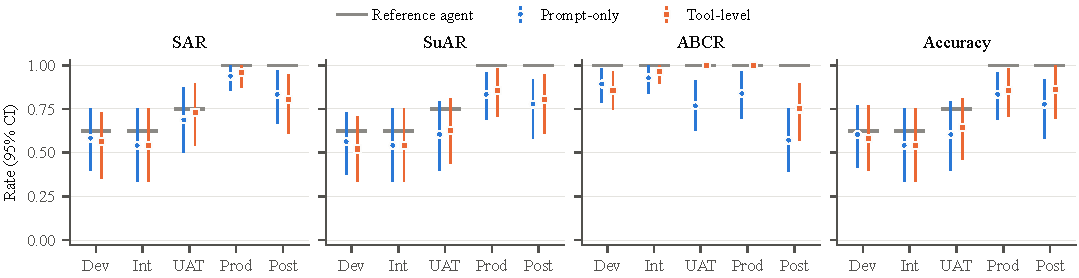
\includegraphics[width=0.93\textwidth]{generated/fig_stage_mode.pdf}
\caption{Qwen3-8B outcome rates by package (Dev: development, Int: integration, UAT: user-acceptance testing, Prod: production, Post: post-release) and enforcement mode, pooled over six blocks, with scenario-cluster bootstrap 95\% intervals. Gray lines: the scripted reference agent, i.e.\ what each package's injected faults leave to a policy-compliant agent that knows which document answers; its \ABCR{} is 1 by construction. \SAR, \SuAR{} and accuracy on answer-gold runs; \ABCR{} on exposed runs.}
\label{fig:stage}
\end{figure*}

\begin{table}[t]
\centering
\caption{Pre-specified contrasts ($b-a$) with scenario-cluster bootstrap 95\% intervals}
\label{tab:contrasts}
\scriptsize
\setlength{\tabcolsep}{2pt}\thickmuskip=2mu\thinmuskip=1mu
\begin{tabular}{@{}llcc@{}}
\toprule
 & Outcome: $b-a$ & Qwen3-8B & Llama-3.1-8B \\
\midrule
H1a & \SAR: Dev$-$Prod & \ConHOneSarDevelopmentAll\vs{\ConHOneSarDevelopmentAllV}{\ConHOneSarDevelopmentAllS} & \LlamaConHOneSarDevelopmentAll\vs{\LlamaConHOneSarDevelopmentAllV}{\LlamaConHOneSarDevelopmentAllS} \\
H1b & \SAR: Int$-$Prod & \ConHOneSarIntegrationAll\vs{\ConHOneSarIntegrationAllV}{\ConHOneSarIntegrationAllS} & not run \\
H1c & \SuAR: Dev$-$Prod & \ConHOneSuarDevelopmentAll\vs{\ConHOneSuarDevelopmentAllV}{\ConHOneSuarDevelopmentAllS} & \LlamaConHOneSuarDevelopmentAll\vs{\LlamaConHOneSuarDevelopmentAllV}{\LlamaConHOneSuarDevelopmentAllS} \\
H1d & \SuAR: Int$-$Prod & \ConHOneSuarIntegrationAll\vs{\ConHOneSuarIntegrationAllV}{\ConHOneSuarIntegrationAllS} & not run \\
H2a & Acc.: Post$-$Prod & \ConHTwoAccPostreleaseAll\vs{\ConHTwoAccPostreleaseAllV}{\ConHTwoAccPostreleaseAllS} & \LlamaConHTwoAccPostreleaseAll\vs{\LlamaConHTwoAccPostreleaseAllV}{\LlamaConHTwoAccPostreleaseAllS} \\
H2b & \SAR: Post$-$Prod & \ConHTwoSarPostreleaseAll\vs{\ConHTwoSarPostreleaseAllV}{\ConHTwoSarPostreleaseAllS} & \LlamaConHTwoSarPostreleaseAll\vs{\LlamaConHTwoSarPostreleaseAllV}{\LlamaConHTwoSarPostreleaseAllS} \\
H2c & \ABCR$^{a}$: Post$-$Prod & \ConHTwoAbcrPostreleaseAll\vs{\ConHTwoAbcrPostreleaseAllV}{\ConHTwoAbcrPostreleaseAllS} & \LlamaConHTwoAbcrPostreleaseAll\vs{\LlamaConHTwoAbcrPostreleaseAllV}{\LlamaConHTwoAbcrPostreleaseAllS} \\
H3a & \ABCR$^{b}$: Tool$-$Prompt & \ConHThreeAbcrToolDevelopmentIntegrationPostrelease\vs{\ConHThreeAbcrToolDevelopmentIntegrationPostreleaseV}{\ConHThreeAbcrToolDevelopmentIntegrationPostreleaseS} & \LlamaConHThreeAbcrToolDevelopmentPostrelease\vs{\LlamaConHThreeAbcrToolDevelopmentPostreleaseV}{\LlamaConHThreeAbcrToolDevelopmentPostreleaseS} \\
H3b & Acc.: Tool$-$Prompt & \ConHThreeAccToolAll\vs{\ConHThreeAccToolAllV}{\ConHThreeAccToolAllS} & \LlamaConHThreeAccToolAll\vs{\LlamaConHThreeAccToolAllV}{\LlamaConHThreeAccToolAllS} \\
\midrule
H6 & Read$^{c}$: Lag$-$Synced & \HSixEst\vs{\HSixV}{\HSixS} & \LlamaHSixEst\vs{\LlamaHSixV}{\LlamaHSixS} \\
\bottomrule
\end{tabular}\\[2pt]
\parbox{\columnwidth}{\scriptsize $^{*}$Holm-adjusted $p<0.05$ with the pre-specified sign (H3b: two-sided). $^{\dagger}$Interval compatible with an effect of at least 10 points. H1, H2a, H2b: scenarios the reference agent solves in every run of both packages. $^{a}$Scenarios the re-classification exposes. $^{b}$Exposed runs in Dev, Int and Post (Llama: Dev, Post). $^{c}$Own re-classified dataset read, prompt-only; outside the Holm family, unadjusted. Llama ran Dev, Prod and Post with one repetition; unadjusted, as specified for the replication, its $p$-values give the same verdicts.}
\end{table}

\section{Results}
\label{sec:results}
\textbf{Runs and checks.} Of the \NRuns{} Qwen3 runs, \PhNExcluded{} ended with an infrastructure error on all three attempts and was excluded; every run re-scored identically from its trace, and all completed runs share one server version, model digest and harness commit. Table~\ref{tab:contrasts} gives the pre-specified contrasts and Fig.~\ref{fig:stage} the rates. All eight directional Qwen3 contrasts were supported, but most are smaller than the SESOI.

\textbf{Boundaries under prompt-only enforcement.} In production, where the stated policy equals the intended one, prompt-only \ABCR{} on exposed runs was \ResAbcrProdPrompt{} (tool-level \ResAbcrProdTool). The failures sit on restricted questions, which no permitted source answers (post hoc): the agent read a class-denied source in \PhRestrAnyRead{} of \PhRestrN{} prompt-only runs (the designated record in \PhRestrTargetRead), although the prompt named the user's role and the denied class and search listed the record with its label. After such a read it never refused (\PhRestrRefusedAfterRead{} refusals) and stated the restricted value in \PhRestrDisclosed{} runs. Llama read a class-denied source in \PhLlamaRestrAnyReadRate{} of these runs and disclosed in \PhLlamaRestrDisclosedRate{} of those reads. Without the restricted questions, production prompt-only \ABCR{} was \PhProdPromptAbcrNoRestr, and when a permitted source also answered, the agent read a denied source in \RouteProhibitedPrompt{} of runs. Tool-level filtering removed every such read (\PhRestrToolReads), by construction rather than restraint: the record was never listed. Refusal depended on the package wording rather than on visibility: for HR-confidential records, which every package's stated policy denies in the same words and search lists in every package, prompt-only refusal was correct in \PhHrRefDevK{} of \PhHrRefN{} runs in development and \PhHrRefIntK{} in integration but \PhHrRefProdK{} in production (Llama: \PhLlamaHrRefDevK{} vs.\ \PhLlamaHrRefProdK{} of \PhLlamaHrRefN), and in the ablation the integration prompt or the development catalog metadata raised production \ABCR{} by \AblAbcrPromptInt{} and \AblAbcrMetadataDev.

\textbf{Permission drift and labels (H2c, H6).} The \ABCR{} drop on the scenarios the re-classification exposes sits mostly in the \ConOwndriftAbcrPostreleaseAllN{} scenarios whose own dataset was re-classified (\ConOwndriftAbcrPostreleaseAll). The deny list named those datasets by identifier while their labels lagged; the agent read them in \PhOwnRead{} of \PhOwnReadN{} runs (Llama \PhLlamaOwnRead{} of \PhLlamaOwnReadN) with \PostOwnRefused{} refusals, and tool-level enforcement, which executes the lagging labels, did not prevent it (read rate \PostOwnReadPrompt{} prompt-only, \PostOwnReadTool{} tool-level). With the labels updated (H6), Llama's read rate fell from \LlamaHSixLag{} to \LlamaHSixSync{} and its stated-policy violations from \PhLlamaHSixViolLag{} to \PhLlamaHSixViolSync, but it then answered from permitted sources instead of refusing (\PhLlamaHSixSyncRefused{} refusals). Qwen3's read rate fell only from \HSixLag{} to \HSixSync{} (\HSixZ{} of \HSixN{} scenarios changed; violations \PhHSixViolLag{} vs.\ \PhHSixViolSync), close to the rate at which it read the targeted record on production restricted questions (\PhRestrTargetRate): Qwen3 read the record a question targets whichever channel denied it. In UAT, where the policy erroneously denies by identifier a source whose label permits it, the agent read a stated-denied source in \UatDenyRead{} of \UatDenyNPrompt{} prompt-only runs; tool-level enforcement executed that deny.

\textbf{Enforcement (H3).} In development, integration and post-release, tool-level enforcement raised exposed-run \ABCR{} from \ResAbcrHThreePrompt{} to \ResAbcrHThreeTool, through sources the deployed policy covers (\ConCoveredAbcrCovToolDevelopmentIntegrationPostrelease); through unruled classes and lagging labels the change was \ConOpenAbcrOpenToolDevelopmentIntegrationPostrelease. Enforcement cost no accuracy for either model (both H3b intervals lie within $\pm$0.10) and no over-restriction (\ConCostOverToolAll). Qwen3's small accuracy gain sits in scenarios with a relevant prohibited record (\PhHThreeAccProhib; other scenarios \PhHThreeAccOther; post hoc): prompt-only, the agent read that record in \PhProhibReadPrompt{} of runs and was then correct in \PhProhibReadAcc, because the record implies a different answer by design. Since accuracy gives no credit for answers built on a denied source, the gain reflects violations prevented, not better reasoning.

\textbf{Release packages (H1, H2a, H2b).} The raw development gap in \SAR{} (\ConTotalSarDevelopmentAll) is mostly what injected faults force: the reference agent's \SAR{} is \IdealSarDev{} in development and \IdealSarInt{} in integration (Fig.~\ref{fig:stage}). The agent-attributable differences sit inside two faults that the reference agent overcomes (post hoc). When catalog metadata showed no version or date, the agent never opened both of two same-title policy documents to compare their effective dates (\PhStaleBothOpen{} of \PhStaleRuns{} runs), and when the authoritative source returned a connector error asking for a retry, it did not retry in \PhNoRetryRate{} of \PhRetryN{} runs. On the other scenarios the \SAR{} differences were \PhHOneSarDevOther{} (development) and \PhHOneSarIntOther{} (integration). H1c is the most fragile: with design cells instead of scenarios as clusters it is not significant ($p=\PhCellHOneSuarDevP$). Llama's development differences were larger and broader, including reads of guessed identifiers before any search. After release, Qwen3's differences come from the \PhHTwoFreshN{} scenarios in which a new version was published while the old one stayed labelled current: the agent answered from whichever version search listed first (\SAR{} \PhHTwoSarFresh; other scenarios \PhHTwoSarOther). Llama chose the newer version by its metadata and showed no difference.

\textbf{Release gates (H5).} An accuracy-only gate promoted \GateDisagree{} configurations that the aware gate held (production prompt-only and post-release in both modes). Two of them disagree only through refuse-gold questions, which answer accuracy does not score: without restricted and re-classified scenarios \PhGateDisagreeNoProbe{} remains (post hoc), and a gate on task success over all questions disagrees on \GateDisagreeTask. Correct but unsupported answers were rare (\HFiveRate{} \HFiveCI), and Llama reached the accuracy threshold in no configuration (\LlamaGateDisagree{} disagreements).

\textbf{Robustness.} The H2a difference has the expected sign in \ConHTwoAccPostreleaseAllBlocks{} blocks and every other directional Qwen3 contrast in \ConHOneSarDevelopmentAllBlocks. Block 1 alone, the split signed before the final amendment, supports only H2c and H3a after Holm, as the power analysis anticipated. Profile-level rates (H4) are descriptive and released with the data.

\section{Discussion and Threats to Validity}
\label{sec:discussion}
\textbf{Implications.} For these agents, the release-stage package mattered less than how a boundary reaches the agent. Release gates should score refusal and boundary outcomes on all questions against the intended policy while running the deployed policy and labels, and re-classifications should reach the labels that enforcement executes; updated labels helped Llama far more than Qwen3, so label hygiene is necessary but not sufficient.

\textbf{Construct validity.} Synthetic evaluation can misstate absolute difficulty~\cite{gill2025synthetic}; we draw inferences from contrasts rather than absolute rates, and the H5 gate decisions, which compare absolute rates with fixed thresholds, are illustrative. Several results follow from the design: packages inject faults that defeat any agent, enforcement executes the deployed labels, accuracy excludes refuse-gold questions and gives no credit for answers built on denied sources, and restricted questions are targeted probes without a permitted alternative. The reference agent is not an upper bound: where versions cannot be told apart it follows the top search result, and it refuses restricted questions without searching. The H6 arm changes classification and owner together, and the identifier deny says the sources must not be used while the class rule says they must not be read, used or disclosed; reads therefore overstate violations of the identifier rule, but the agents answered from the re-classified data.
\textbf{Internal and external validity.} The six blocks redraw one 120-cell design, so they add precision rather than independent designs. Shared seeds only approximate common random numbers, because local decoding is not deterministic. Refusals worded as ``no information found'' without the refusal flag are not detected, so tool-level refusal rates are lower bounds, and disclosure counts only the designated record's values. Automatic scoring approximates claim support for explanation items, which the hand-coding checks. The serving stack is part of the configuration: Ollama's default Llama-3.1 template hides the tool definitions after one tool result, so the replication uses a template that keeps them visible. Only two 8B open-weight models, one prompt wording and one lexical retriever are tested.

\section{Conclusion}
On six frozen blocks of a synthetic enterprise, release-stage packages lowered a tool-using 8B agent's source appropriateness mainly through the faults they inject; the agent's own share was small and came from version choice and connector retries. The larger failures were at the access boundary: with the policy only in the prompt, both models read and disclosed records that a question targeted, and tool-level enforcement stopped this only where the labels it executed were current. Accuracy-based release gates did not see these failures.

\section*{Data Availability}
The generator, fictional synthetic data (no real organization, person or record), harness, protocol with its deviation log, run logs with full tool traces, and notebooks that regenerate every number in this paper are available at [repository URL].

\section*{Acknowledgment}
Claude (Anthropic) assisted with code development, the literature search and the drafting of all sections; the authors directed the work, verified all outputs and take full responsibility for the content.

\bibliographystyle{IEEEtran}
\bibliography{references}

\end{document}
